\documentclass[12pt,a4paper]{book}

\setcounter{tocdepth}{3}

\usepackage[utf8]{inputenc}
\usepackage[french]{babel}
\usepackage[T1]{fontenc}
\usepackage{graphicx}
\usepackage{fullpage}
\usepackage{url}
\usepackage{adjustbox}

\usepackage{amsmath}
\usepackage{amsfonts}
\usepackage{dsfont}
\usepackage{amssymb}

\usepackage{comment}

\usepackage{amsthm}
\newtheorem{env_definition}{Définition}
\newtheorem{formule}{Formule}
\newtheorem{annexe}{Annexe}

\usepackage[colored]{shadethm}
\definecolor{shadethmcolor}{rgb}{1,0.871,0.890}% couleur du fond
\definecolor{shaderulecolor}{rgb}{0.651,0.074,0.090}% couleur de l'encadré
\newshadetheorem{env_proposition}{Proposition}
\newshadetheorem{env_lemme}{Lemme}
\newshadetheorem{theorem}{Théorème}

\newcommand{\R}{\mathbb{R}}

\renewcommand\thesection{\Roman{section}}

\newcommand{\E}{\mathbb{E}}
\newcommand{\p}{\mathbb{P}}
\newcommand{\1}{\mathds{1}}

\DeclareMathOperator*{\argmin}{arg\!\min}


\usepackage{pythonhighlight}
%\usepackage[margin=0.5in]{geometry}
\usepackage{color, colortbl}
\usepackage{xcolor}
\usepackage{graphicx}
\usepackage{caption}



\definecolor{Gray}{gray}{0.9}
\definecolor{DarkGray}{gray}{0.5}
\definecolor{LightCyan}{rgb}{0.88,1,1}
\definecolor{yellow}{rgb}{1,1,0}


\begin{document}



% Page de garde
	
\begin{titlepage}
	\thispagestyle{empty}
	\begin{center}
	
    
\includegraphics[scale=1.]{Logo}  
	\vspace{1 cm}

	{\fontsize{25}{30} \selectfont Travail encadré de recherche :}\\
	\vspace{0.7 cm}
	\textbf{{\fontsize{30}{35} \selectfont Profilage des consommateurs à l'aide des k-means++ semi-supervisés}}\\
	\vspace{1 cm}
	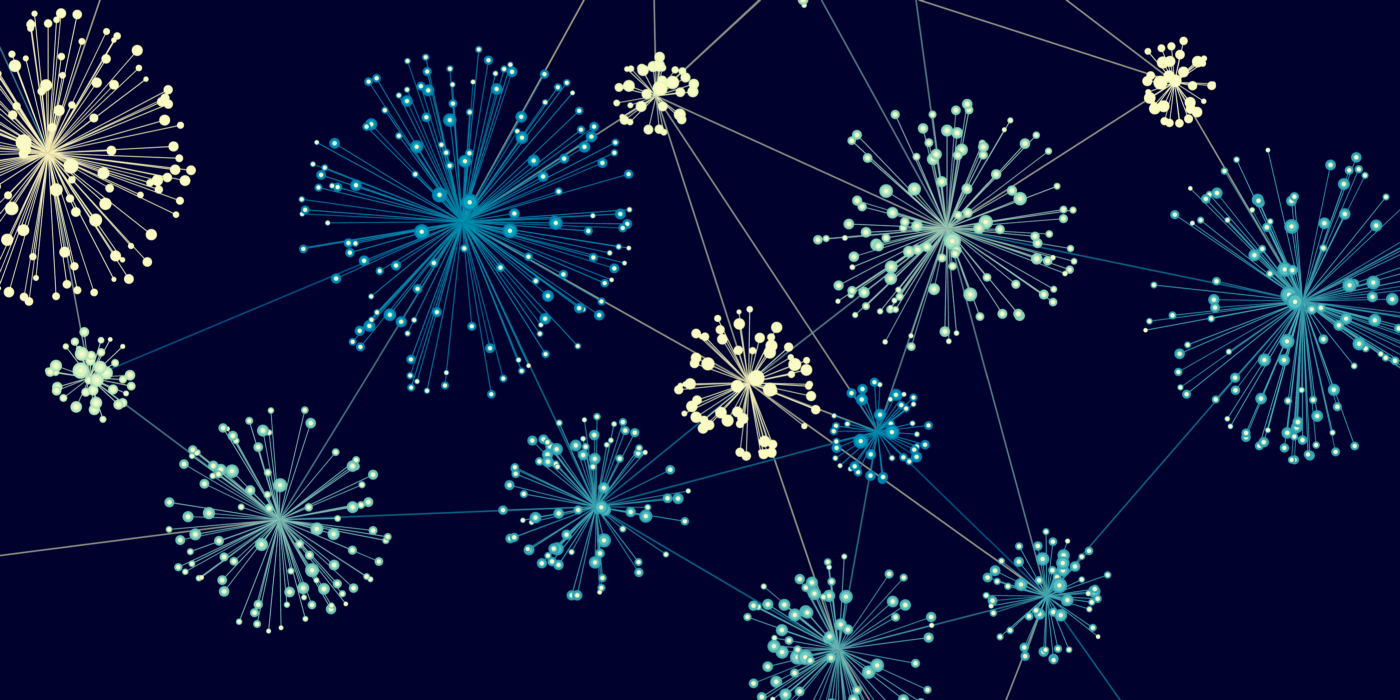
\includegraphics[width=11 cm]{image1}  
	
	\vspace{1.5 cm}
	{\fontsize{15}{25} \selectfont Par : \\
		\item Destin ASHUZA CIRUMANGA
		\item Elvina GOVENDASAMY
	}\\
	\vspace{0.5 cm}
	{\fontsize{15}{25} \selectfont Master 1 Mathématiques et Applications}\\
	{\fontsize{15}{25} \selectfont Parcours Data Science}\\
	\vspace{1 cm}
	{\fontsize{15}{25} \selectfont Sous la direction de Mme Eunice OKOME OBIANG}
	\vspace{1.5 cm}

	{\fontsize{20}{30} \selectfont 2019-2020}\\
	
	\end{center}
\end{titlepage}

\thispagestyle{empty}
\newpage
~


% Description du sujet

\newpage
\setcounter{page}{1}

\noindent
{\LARGE \textbf{Description}}
\vspace{5 mm}

\noindent
La segmentation des populations est un problème rencontré dans de  nombreuses disciplines. En marketing par exemple, cette technique permet aux entreprises d'identifier et de caractériser les différents profils de consommateurs, afin de leur offrir des produits et des services adaptés à  leurs besoins.\\

\noindent
Le clustering par l'algorithme des k-means est la méthode d'apprentissage non supervisé la plus utilisée pour répondre à ce type de problématique. Son objectif est de segmenter la population en $k$ groupes disjoints sur base d'un critère de similarité. Toutefois, la qualité de ce modèle varie selon le choix des centres initiaux des clusters. L'idée des k-means++ semi supervisés est de contrôler l'initialisation des centres de clusters en intégrant des données supervisées dans le processus d'apprentissage pour ainsi améliorer les performances du clustering en termes de coût et de durée d'exécution.\\

\noindent
Dans ce travail, nous nous intéressons dans un premier temps à la présentation de différents résultats théoriques sur les différents algorithmes des k-means et à la démonstration d'un critère de qualité associé aux k-means++ semi-supervisés. Dans un second temps, nous programmons et testons l'algorithme des k-means++ semi-supervisés sur un jeu de données clients.

% Table des matières

\tableofcontents
\newpage
~



% Contenu du rapport

\newpage

% #######################################################################################
% #######################################################################################

\section*{Introduction}
\addcontentsline{toc}{section}{Introduction}

A l'ère du big data et de l'intelligence artificielle, le recours aux outils d'analyse et d'exploitation des données est de plus en plus fréquent, et ce dans tous les secteurs désormais. L'apprentissage statistique - machine learning en anglais - est la science au cœur de l'exploitation de ces données et de l'automatisation des méthodes dévolues à cette fin. Il existe différents types d'apprentissage, chacun ayant ses points forts et ses inconvénients. La distinction la plus courante se fait entre l'apprentissage supervisé et l'apprentissage non supervisé qui regroupent la plupart des problèmes. Et un mariage entre ces deux types donne l'apprentissage semi-supervisé. 

Dans l'apprentissage supervisé, l'on dispose de $p$ variables notées $X$ mesurées sur $n$ individus et d'une variable réponse notée $Y$. L'objectif est de trouver une relation entre les variables explicatives $X$ permettant d'approcher au mieux la vraie réponse $Y$. Les avantages de cet apprentissage sont entre autres des résultats facilement interprétables, de meilleures performances prédictives ou encore des modèles facilement comparables. Cependant l'acquisition de l'information a un coût. En effet, l'information contenue dans la variable réponse nécessite une mobilisation des moyens pour son obtention. Nous pouvons penser à des questionnaires d'enquêtes ou l'embauche du personnel supplémentaire pour s'en occuper. De plus, dans la catégorisation des individus, il n'est pas impossible que l'humain y insère un biais pour telle ou telle autre raison.

Quant à l'apprentissage non supervisé, la variable réponse n'est plus disponible. Le but sera alors d'identifier des patterns ou des relations entre les variables, de regrouper les individus présentant des similitudes (clustering) ou encore de mettre en évidence les variables les plus significatives. L'inconvénient majeur de ce type d'apprentissage est la difficulté à interpréter les modèles ou à évaluer leurs performances.  Mais il a comme avantages une facilité de mise en œuvre, des coûts réduits pour l'acquisition de l'information et une possible correction du biais qui serait dû aux a priori sur la catégorisation des individus.

Pour ce qui est de l'apprentissage semi-supervisé, il est obtenu comme un jumelage de deux types précédents : l'on dispose de l'information $Y$ juste pour une partie des données. Dès lors, ses avantages sont un mélange entre les avantages du supervisé et du non supervisé : la correction du biais sur les catégories, des performances significatives par rapport au non supervisé et augmentant avec la quantité des données supervisées, l'acquisition de l'information moins coûteuse par rapport au supervisé. Toutefois, dans certains cas, l'interprétation du modèle pose toujours problème.

L'algorithme des k-means qui fait l'objet de ce travail est un algorithme simple et très utilisé relevant de l'apprentissage non supervisé. Dans une première partie théorique, nous présentons cet algorithme et son principe de fonctionnement ; ensuite nous présentons sa version améliorée, les k-means++, en démontrant un critère de qualité qui lui est associé ; et enfin nous étendons cette dernière version au cas où l'on dispose de certaines données qui sont labellisées, ce qui donne l'algorithme des k-means++ semi-supervisés. Dans une deuxième partie appliquée, nous implémentons ces algorithmes grâce au langage python et nous les testons sur une base réelle des données clients. Il en résulte que les k-means++ semi supervisés sont de loin plus performants.




% #######################################################################################
% #######################################################################################

\section{Partie théorique}

Cette partie est consacrée à la présentation et à l'étude théorique de différents algorithmes de k-means. Les  résultats énoncés et démontrés sont essentiellement tirés de \cite{DAV2007} et de \cite{JOR2017}. Ils sont suffisamment détaillés pour être facilement accessibles à toute personne ayant des bases en probabilités et en statistique.

\subsection{Les k-means standards}

\subsubsection{Présentation de l'algorithme}

L'algorithme des k-means est utilisé pour résoudre le problème suivant : étant donné un entier natural $k$ fixé et un ensemble de points $X \subset \R^d$ (avec $d \geq 1$), trouver un ensemble de centres $C = \{ c_i \in \R^d, i=1,2,...,k \}$ tel que 
\begin{equation}\label{probleme_kmeans}
	C = \argmin_{\{ A \subset \R^d, card(A)=k \}}\sum_{x \in X} \min_{c \in A} \Vert x-c \Vert^2
\end{equation}
Par la suite, en utilisant ces centres, le label de chaque élément $x$ est donné par :
$$
	\ell (x) = \argmin_{1 \leq i \leq k} \Vert x - c_i \Vert
$$

Résoudre l'équation (\ref{probleme_kmeans}) de manière exacte pour trouver $C$  est "NP-hard" ; c'est-à-dire qu'il est difficile de trouver une solution exacte avec un algorithme de complexité polynomiale. Ainsi, en pratique, l'on se contente d'approcher la solution de manière locale. L'algorithme de Lloyd est le plus utilisé pour cette fin. Il prend en entrée l'ensemble des données $X$, les centres initiaux $C$  et retourne les centres finaux résolvant localement l'équation (\ref{probleme_kmeans}). Concrètement, on l'implémente comme suit :  \\

\noindent \textbf{\underline{Algorithme de Lloyd}}\label{algo_lloyd}

\noindent \textbf{Entrées : } $X$ (le dataset) et $C$ (l'ensemble des $k$ centres initiaux)\\
\noindent \textbf{Sorties : } $C$ (l'ensemble des centres définitifs) \\
\textbf{1} \textbf{faire}\\
\textbf{2} \indent associer chaque $x_i \in X$ au centre le plus proche $c(x_i) \in C$\\
\textbf{3} \indent remplacer chaque $c_j \in C$ par le point moyen des $x \in X$ tels que $c(x)=c_j$\\
\textbf{4} \textbf{jusqu'à ce que } $C$ ne change plus\\
\textbf{5} \textbf{sortir} $C$ \\

L'algorithme des k-means standards est alors obtenu en exécutant l'algorithme de Lloyd avec les centres initiaux qui sont choisis uniformément dans $X$
\subsubsection{Convergence}

Après avoir compris le fonctionnement de l'algorithme de Lloyd (et donc celui des k-means standards qui en découle), une question légitime se pose : l'algorithme s'arrête-t-il ?\\ Avant de répondre à cette question, introduisons d'abord quelques définitions et notations qui nous seront utiles dans la suite de ce travail.

	\begin{env_definition}\label{clustering}
		\textbf{(Clustering)}\\
		Un clustering $C$ est un ensemble de centres qui sont utilisés pour déterminer le label de chaque point du jeu de données $X$.
	\end{env_definition}
	
	\begin{env_definition}\label{fonction_potentielle}
		\textbf{(Fonction potentielle)}\\
		Étant donné un clustering $C$ , la fonction potentielle $\phi$ associée à $C$ est la fonction à valeurs dans $\R^+$ définie dans l'ensemble des parties de $X$ par :
		$$
			\forall A \subset X \,, \quad \phi(A) = \sum_{a \in A} \min_{c \in C} \Vert a - c \Vert^2
		$$
		Par la suite, par abus de notation, l'on écrira tout simplement $\phi(X) = \phi$ et uniquement pour $X$.
	\end{env_definition}
	
	\begin{env_definition}\label{clustering_optimal}
		\textbf{(Clustering optimal et cluster optimal)}\\
		Soit $C_{OPT}$ le clustering qui serait la solution exacte du problème des k-means tel que formulé par l'équation (\ref{probleme_kmeans}) à la page \pageref{probleme_kmeans}. $C_{OPT}$ sera alors appelé clustering optimal et tout cluster dans $C_{OPT}$ sera appelé cluster optimal.
	\end{env_definition}
	
	\begin{env_definition}\label{poids_d}
		\textbf{(Poids $D^2$)}\\
		Étant donné un clustering $C$, le poids $D^2$ est défini par :
		$$
			\forall x \in X \,, \quad D^2(x) = \phi(\{x\}) = \min_{c \in C} \Vert x - c \Vert^2
		$$
		C'est donc le carré de la distance de $x$ au centre dans $C$ qui lui est le plus proche.
	\end{env_definition}
	
	A la lumière de ces définitions, nous pouvons résumer le problème de k-means comme suit :
	\begin{itemize}
		\item Le problème de k-means tel que formulé par l'équation (\ref{probleme_kmeans}) à la page \pageref{probleme_kmeans} consiste à trouver le clustering qui minimise la fonction potentielle $\phi$
		\item Théoriquement, on sait qu'il existe une solution exacte $C_{OPT}$ à ce problème mais en pratique il est difficile de la calculer.
		\item L'algorithme des k-means fait donc appel à l'algorithme de Llyod (donné à la page \pageref{algo_lloyd}) pour trouver un minimum local de $\phi$ atteint en une solution approchée donnée par un clustering $C$. \\
	\end{itemize}

Nous pouvons maintenant énoncer le résultat qui nous permet d'affirmer que l'algorithme s'arrête :

	\begin{env_lemme}\label{lemme2.1}
		Soient $S$ un ensemble de points, $c(S)$ son point moyen (son centre de gravité, son isobarycentre) et $z$ un point quelconque.\\
		Alors, on a :
		
		$$
			\sum_{x \in S} \; \Vert x-z \Vert^2 - \sum_{x \in S} \; \Vert x-c(S) \Vert^2 = card(S) \cdot \Vert c(S)-z \Vert^2
		$$
		où $card(S)$ désigne le cardinal de $S$.
	\end{env_lemme}	
	
	\begin{proof}
		~\\
		Nous avons :
		\begin{eqnarray*}
			\sum_{x \in S} \; \Vert x-z \Vert^2 &=& \sum_{x \in S} \; \Vert \left( x - c(S) \right) + \left( c(S)- z \right) \Vert^2 \\
			& = & \sum_{x \in S} \; \Vert x - c(S) \Vert^2 + 2 \cdot \sum_{x \in S} \; \langle x - c(S), \; c(S)- z \rangle + \sum_{x \in S} \; \Vert c(S)- z \Vert^2 \\
			& = & \sum_{x \in S} \; \Vert x - c(S) \Vert^2 + 2 \cdot \langle \sum_{x \in S} \; x - card(S) \cdot c(S), \; c(S)- z \rangle + card(S) \cdot \Vert c(S)- z \Vert^2 \\
			& = & \sum_{x \in S} \; \Vert x - c(S) \Vert^2 + 2 \cdot card(S) \cdot \langle c(S) - c(S), \; c(S)- z \rangle + card(S) \cdot \Vert c(S)- z \Vert^2 \\
			& = & \sum_{x \in S} \; \Vert x - c(S) \Vert^2 + 2 \cdot card(S) \cdot \langle 0, \; c(S)- z \rangle + card(S) \cdot\Vert c(S)- z \Vert^2 \\.
			& = & \sum_{x \in S} \; \Vert x - c(S) \Vert^2 + card(S) \cdot \Vert c(S)- z \Vert^2
		\end{eqnarray*}
		d'où le résultat.
	\end{proof}

Le lemme \ref{lemme2.1} nous permet d'affirmer que remplacer le centre de chaque cluster par le point moyen de ses éléments à chaque tour de boucle de l'algorithme de Llyod permet de décroître nécessairement $\phi$. Ainsi dès que $\phi$ atteint un minimum local, l'algorithme s'arrête.

Nous pourrions être content de savoir que l'algorithme s'arrête toujours. Malheureusement rien ne garantit que la solution locale obtenue donne un bon clustering. En effet, $\phi$  peut être arbitrairement grand malgré l'optimum local atteint. C'est le défaut principal de l'algorithme des k-means standards. Dans la section suivante, nous présentons les k-means++ qui résolvent ce problème.

%===============================================================================

\subsection{Les k-means++}

\subsubsection{Présentation de l'algorithme}

L'algorithme des k-means++ est obtenu en changeant uniquement la manière dont sont initialisés les centres initiaux qui seront utilisés dans l'algorithme de Lloyd. Au lieu de les choisir uniformément, ces centres initiaux sont choisis avec une probabilité proportionnelle au poids $D^2$. Ensuite le reste se passe exactement comme pour les k-means standards en faisant appel à l'algorithme de Lloyd. Voici l'algorithme d'initialisation en question : \\

\noindent \textbf{\underline{Algorithme d'initialisation des centres pour les k-means++}}\label{algo_kmeans_pp}

\noindent \textbf{Entrées : } $X$ (le dataset) et $k$ (le nombre de centres)\\
\noindent \textbf{Sorties : } $C$ (l'ensemble des centres initiaux) \\
\textbf{1} choisir un $x \in X$ suivant la loi uniforme\\
\textbf{2} initialiser $C=\{x\}$\\
\textbf{3} \textbf{Tant que } $card(C) \leq k$ \textbf{faire}\\
\textbf{4} \indent choisir un $x \in X$ avec probabilité proportionnelle à $D^2(x)$\\
\textbf{5} \indent actualiser $C = C \cup \{x \}$\\
\textbf{6} \textbf{sortir} $C$ \\

\subsubsection{Critère de qualité}

Dans cette section, nous présentons les résultats qui montrent que l'algorithme des k-means++ est meilleur que celui des k-means standards dans le sens où l'espérance de la fonction potentielle est majorée. Plus exactement, le théorème \ref{theoreme3.1} présenté à la fin de cette section montre que la fonction potentielle obtenue à fin de l'étape de l'initialisation de l'algorithme des k-means++ est un $O(\ln k)$ par rapport au clustering optimal théorique. Et cela est suffisant car dans l'algorithme de Lloyd, cette fonction ne peut faire que baisser.

Nous présentons trois lemmes qui permettent de démontrer le théorème en question : le premier permet de contrôler $\phi$ pour le choix du premier centre ; le deuxième montre que $\phi$ reste toujours majorée lorsque l'on choisit les centres restants dans les clusters optimaux théoriques proportionnellement au poids $D^2$. Enfin le troisième lemme généralise cela pour n'importe quel choix des centres, ce qui conduit à la démonstration du théorème.

	\begin{env_lemme}\label{lemme3.1}
		Soient $A$ un cluster arbitraire dans $C_{OPT}$ et $c(A)$ son point moyen. Soit $C$ un clustering avec un unique centre choisi aléatoirement dans $A$ et de fonction potentielle $\phi$.\\
		Alors, on a :
		
		$$
			\E\left[\phi(A)\right] = 2 \cdot \phi_{OPT} \left( A \right)
		$$		
	\end{env_lemme}	
	
	\begin{proof}
		~\\
		Supposons que $C=\{ a_0 \}$  avec $a_0$ qui a été choisi aléatoirement dans A ; c'est-à-dire :
		$$
			\p \left( \{ choisir \; a_0  \} \right) = \frac{1}{card(A)}
		$$
		
		En faisant varier le choix de $a_0$, nous voyons clairement que $\phi(A)$ est une variable aléatoire discrète à valeurs dans $\R$. En effet, $card\left(\phi(A)\left(\Omega\right)\right) = card(A)$ et pour chaque choix de $a_0$, la valeur prise par $\phi(A)$ est donnée par :
		\begin{eqnarray*}
			\phi_{a_0}(A) &=& \phi\left(A;C\right) \\
			&=& \phi\left(A;\{a_0\}\right) \\
			&=& \sum_{a \in A} \min_{c \in \{ a_0 \}} \Vert a - c \Vert^2 \\
			&=& \sum_{a \in A} \Vert a - a_0 \Vert^2
		\end{eqnarray*}
		
		De plus, par le lemme \ref{lemme2.1} énoncé à la page \pageref{lemme2.1}, nous savons que le point moyen $c(A)$ du cluster $A$ est nécessairement le centre utilisé pour ce cluster dans le clustering optimal $C_{OPT}$ sinon $\phi_{OPT}$ ne serait pas minimale.
		De tout ce qui précède, nous pouvons alors écrire :
		\begin{eqnarray*}
			\E\left[\phi(A)\right] &=& \sum_{a_0 \in A} \phi_{a_0}(A) \cdot \p \left( \phi(A)= \phi_{a_0}(A) \right) \\
			&=& \sum_{a_0 \in A} \left( \sum_{a \in A} \Vert a-a_0 \Vert^2 \cdot \frac{1}{card(A)} \right) \\
			&=& \frac{1}{card(A)} \cdot \sum_{a_0 \in A} \sum_{a \in A} \Vert a-a_0 \Vert^2
		\end{eqnarray*}
		En appliquant le lemme \ref{lemme2.1} avec $S=A$ et $z=a_0$, nous obtenons :
		\begin{eqnarray*}
			\E\left[\phi(A)\right] &=& \frac{1}{card(A)} \sum_{a_0 \in A} \left( card(A) \cdot \Vert c(A)-a_0 \Vert^2 + \sum_{a \in A} \Vert a - c(A) \Vert^2 \right) \\
			&=& \sum_{a_0 \in A} \Vert c(A)-a_0 \Vert^2 + \frac{1}{card(A)} \cdot \sum_{a_0 \in A} \sum_{a \in A}\Vert a - c(A) \Vert^2 \\
			&=& \sum_{a_0 \in A} \Vert c(A)-a_0 \Vert^2 + \frac{1}{card(A)} \cdot card(A) \cdot \sum_{a \in A}\Vert a - c(A) \Vert^2 \\
			&=& 2 `\cdot \sum_{a \in A} \Vert c(A) - a \Vert^2 \\
			&=& 2 \cdot \phi_{OPT}(A)
		\end{eqnarray*}
		ce qui conclut la preuve.
	\end{proof}

\begin{env_lemme}\label{lemme3.2}
		Soient $A$ un cluster arbitraire dans $C_{OPT}$ et $C$ un clustering quelconque. Supposons que l'on ajoute aléatoirement un centre à $C$ choisi dans $A$ avec une probabilité proportionnelle à $D^2$, la distance euclidienne au carré. Soit $\phi$ la fonction potentielle du clustering ainsi obtenu.\\
		Alors, on a :
		
		$$
			\E\left[\phi(A)\right] \leq 8 \cdot \phi_{OPT} \left( A \right)
		$$		
	\end{env_lemme}	
	
	\begin{proof}
		~\\
		Soit $1 \leq l < k$ (ici $k$ représente le nombre de centres utilisés pour le clustering optimal $C_{OPT}$).\\
		Supposons que $C=\{ c_1, c_2, ..., c_l \}$   et considérons un cluster $A$ dans $C_{OPT}$.\\
		Rappelons que la distance $D^2$ associée au clustering $C$ vérifie :
		$$
			\forall a \in A, D^2(a) = \min_{c \in C} \Vert a-c \Vert^2
		$$
		Soit $a_0 \in A$ choisi avec probabilité $\dfrac{D^2(a_0)}{\displaystyle \sum_{a \in A} D^2(a)}$ \\
		Notons $C(a_0) = C \cup \{ a_0 \}$ et $\phi_{a_0}$ respectivement le clustering et la  fonction potentielle obtenus pour ce choix de $a_0$. Nous pouvons alors écrire : 
		\begin{eqnarray*}
			\E\left[\phi(A)\right] &=& \sum_{a_0 \in A} \phi_{a_0}(A) \cdot \p \left( \phi(A)= \phi_{a_0}(A) \right) \\
			&=& \sum_{a_0 \in A} \sum_{a \in A} \min_{c \in C(a_0) }\Vert a-c \Vert^2 \cdot \frac{D^2(a_0)}{ \sum_{a \in A} D^2(a)} \\
			&=&  \sum_{a_0 \in A} \sum_{a \in A} \min \left( \min_{c \in C }\Vert a-c \Vert^2, \Vert a- a_0 \Vert^2 \right) \cdot \frac{D^2(a_0)}{ \sum_{a \in A} D^2(a)} \\
			&=&  \sum_{a_0 \in A} \sum_{a \in A} \min \left( D^2(a), \Vert a-a_0 \Vert^2 \right) \cdot \frac{D^2(a_0)}{ \sum_{a \in A} D^2(a)}  
		\end{eqnarray*}
		De plus pour tout $a \in A$, nous avons : 
		\begin{eqnarray*}
			D(a_0) &=& \min_{c \in C} \Vert a_0 - c \Vert \\
			& \leq &  \Vert a_0 - c \Vert = \Vert (a_0 - a) + (a - c) \Vert \qquad \forall c \in C \\
			& \leq & \Vert a_0 - a \Vert + \Vert a - c \Vert \qquad \forall c \in C \quad \textrm{ (par inégalité triangulaire)}
		\end{eqnarray*}
		En particulier pour $c_j \in C$ tel que $D(a) = \Vert a - c_j \Vert$ , nous avons :
		$$
			D(a_0) \leq \Vert a_0 - a \Vert + D(a)
		$$
		D'une part, en élevant au carré les membres de cette inégalité, nous obtenons :
		$$
			D^2(a_0) \leq \Vert a_0 - a \Vert^2 + D^2(a) + 2 \cdot \Vert a_0 - a \Vert \cdot D(a)
		$$
		D'autre part,
		\begin{eqnarray*}
			\bigg( \Vert a_0 - a \Vert - D(a)\bigg)^2 & \geq & 0 \\
			\Leftrightarrow \Vert a_0 - a \Vert^2 + D^2(a) & \geq & 2 \cdot \Vert a_0 - a \Vert \cdot D(a)
		\end{eqnarray*}
		Ainsi, nous en déduisons  que
		$$
			\forall a \in A, \quad D^2(a_0) \leq 2 \cdot \Vert a_0 - a \Vert^2 + 2 \cdot D^2(a)
		$$
		En sommant sur toutes les valeurs de $a$, nous obtenons alors 
		$$
			D^2(a_0) \leq \frac{2}{card(A)} \cdot \sum_{a \in A} \Vert a_0 - a \Vert^2 + \frac{2}{card(A)} \cdot \sum_{a \in A} D^2(a)
		$$
		Nous utilisons ensuite cette inégalité pour majorer $D^2(a_0)$ dans l'expression de $\E\left[\phi(A)\right]$ obtenue précédemment, ce qui conduit à 
		\begin{eqnarray*}
			\E\left[\phi(A)\right] & \leq & \frac{2}{card(A)} \cdot \sum_{a_0 \in A} \sum_{a \in A} \min \left( D^2(a), \Vert a-a_0 \Vert^2 \right) \cdot \frac{\sum_{a \in A} \Vert a_0 - a \Vert^2}{ \sum_{a \in A} D^2(a)} \\
			&& + \quad \frac{2}{card(A)} \cdot \sum_{a_0 \in A} \sum_{a \in A} \min \left( D^2(a), \Vert a-a_0 \Vert^2 \right) \cdot \frac{\sum_{a \in A} D^2(a)}{ \sum_{a \in A} D^2(a)} 
		\end{eqnarray*}
		Dans le second membre de cette inégalité, nous utilisons le fait que 
		$$
			\min \left( D^2(a), \Vert a-a_0 \Vert^2 \right) \leq D^2(a)
		$$
		pour le premier bloc, et 
		$$
			\min \left( D^2(a), \Vert a-a_0 \Vert^2 \right) \leq \Vert a-a_0 \Vert^2
		$$
		pour le second bloc, nous obtenons :
		\begin{eqnarray*}
			\E\left[\phi(A)\right] & \leq & \frac{2}{card(A)} \cdot \sum_{a_0 \in A} \sum_{a \in A} \Vert a_0 - a \Vert^2 \\
			&& + \quad \frac{2}{card(A)} \cdot \sum_{a_0 \in A} \sum_{a \in A} \Vert a-a_0 \Vert^2
		\end{eqnarray*}
		C'est-à-dire 
		$$
			\E\left[\phi(A)\right] \leq 4 \cdot \frac{1}{card(A)} \cdot \sum_{a_0 \in A} \sum_{a \in A} \Vert a_0 - a \Vert^2
		$$
		L'expression $\frac{1}{card(A)} \cdot \sum_{a_0 \in A} \sum_{a \in A} \Vert a_0 - a \Vert^2$ est celle que nous avons obtenue pour l'espérance lors de la démonstration du lemme \ref{lemme3.1} à la page \pageref{lemme3.1}. Ainsi, en appliquant le lemme \ref{lemme3.1}, nous obtenons donc
		$$
			\E\left[\phi(A)\right] \leq 8 \cdot \phi_{OPT} \left( A \right)
		$$
		ce qui est le résultat escompté.
	\end{proof}
	
	\begin{env_lemme}\label{lemme3.3}
		Soient $C$ un clustering arbitraire de fonction potentielle $\phi$ et $u > 0$ un entier naturel.
		Choisissons $u$ clusters  non couverts par $C$ dans $C_{OPT}$. Notons $X_u$ l'ensemble des points de ces clusters et $X_c=X-X_u$ son complémentaire. Supposons que nous ajoutons $t \leq u$ centres à $C$ choisis de manière aléatoire proportionnellement au poids $D^2$. Notons $C'$ le nouveau clustering ainsi obtenu et $\phi'$ sa fonction potentielle associée. Alors, on a :
		
		$$
			\E\left[\phi'\right] \leq \bigg( \phi \left( X_c \right) + 8 \cdot \phi_{OPT} \left( X_u \right) \bigg) \cdot \left( 1 + H_t \right) + \frac{u-t}{u} \cdot \phi \left( X_u \right) ;
		$$
		
		avec $H_t = \displaystyle \sum_{i=1}^{t} \frac{1}{i}$ la $t^{\grave{e}me}$ somme partielle de la série harmonique.
	\end{env_lemme}	
	
	\begin{proof}
		Elle se fait par une récurrence à deux niveaux en montrant que si l'inégalité est vérifiée pour les couples d'entiers $(t-1,u)$ et $(t-1,u-1)$, alors elle l'est également pour le couple $(t,u)$.\\
		
		Regardons d'abord de plus près la fonction $\phi'$ et sa relation avec $\phi$ :\\ 
		Notons $c'_1$, $c'_2$, ..., $c'_t$ les t centres ajoutés à $C$. Pour toute partie $A \subset X$, on a alors :
		
		\begin{eqnarray*}
			\phi' \left( A \right) &=& \sum_{x \in A} \; \min_{c' \in C'} \; \Vert x-c' \Vert^2 \\
			&=& \sum_{x \in A} \; \min	\bigg( D^2 \left(x \right),\Vert x-c'_1 \Vert^2 , ... ,\Vert x-c'_t \Vert^2 \bigg) \\
			& \leq & \sum_{x \in A}	D^2 \left(x \right)	= \phi \left( A \right).	
		\end{eqnarray*}
		
		Passons à la démonstration proprement dite maintenant : \\
		\item[-] \underline{Initialisation}: il suffit de vérifier pour $t=0$, $u > 0$ et $t=1$,$u=1$.
		 \item Pour $t=0$, $u>0$ on a :
		 \begin{eqnarray*}		 
			\E\left[\phi'\right] &=& \phi \textrm{ \; \; \; \; \; \; (car $\phi'= \phi$ qui est constante)}\\
			&=&	\phi \left( X_c \right) + \phi \left( X_u \right)	\\
			&=& \bigg( \phi \left( X_c \right) \bigg) \cdot \left( 1 + H_0 \right) + \frac{u-0}{u} \cdot \phi \left( X_u \right) \textrm{\; \; avec $H_0=0$}	\\
			& \leq & \bigg( \phi \left( X_c \right) + 8 \cdot \phi_{OPT} \left( X_u \right) \bigg) \cdot \left( 1 + H_0 \right) + \frac{u-0}{u} \cdot \phi \left( X_u \right)		
		 \end{eqnarray*}
		 \item Pour $t=1$, $u=1$ on distingue deux cas : soit le nouveau centre est choisi dans le seul cluster non couvert, soit il est choisi dans l'un des clusters couverts.\\
		 Si le nouveau centre $c'_1$ est choisi dans le cluster non couvert, il l'est avec probabilité $\dfrac{\phi \left( X_u \right)}{\phi}$ et on a :
		 \begin{eqnarray*}
		 	\phi' &=& \phi' \left( X_c \right) + \phi' \left( X_u \right) \\
		 	& \leq & \phi \left( X_c \right) + \phi' \left( X_u \right)
		 \end{eqnarray*}
		 D'où,
		 \begin{eqnarray*}
		 	\E\left[\phi' \; | \; c'_1 \in X_u \right] & \leq & \phi \left( X_c \right) + \E \left[ \phi' \left( X_u \right) \; | \; c'_1 \in X_u \right] \\
		 	& \leq & \phi \left( X_c \right) + 8 \cdot \phi_{OPT} \left( X_u \right) \textrm{\; \; (par le lemme \ref{lemme3.2}).}
		 \end{eqnarray*}
		 Sinon, le nouveau centre $c'_1$ est choisi dans $X_c$ avec probabilité  $\dfrac{\phi \left( X_c \right)}{\phi}$ et on a :
		 $$
		 	\E\left[\phi' \; | \; c'_1 \in X_c \right] \leq \phi \textrm{ \; \; (car $\phi' \leq \phi$ ).} 
		 $$
		 Finalement,
		 \begin{eqnarray*}
		 	\E\left[\phi'\right] &=& \E\left[\phi' \1_{\{c'_1 \in X_u\}} \right] + \E\left[\phi' \1_{\{c'_1 \in X_c\}} \right] \\
		 	&=& \p \left( c'_1 \in X_u \right)\E\left[\phi' \; | \; c'_1 \in X_u \right] + \p \left( c'_1 \in X_c \right)\E\left[\phi' \; | \; c'_1 \in X_c \right]\\
		 	& \leq & \dfrac{\phi \left( X_u \right)}{\phi} \bigg( \phi \left( X_c \right) + 8 \phi_{OPT} \left( X_u \right) \bigg) + \dfrac{\phi \left( X_c \right)}{\phi} \; \phi \\
		 	& \leq & 2 \cdot  \phi \left( X_c \right) + 8 \cdot \phi_{OPT} \left( X_u \right) \\
		 	& \leq & \bigg( \phi \left( X_c \right) + 8 \cdot \phi_{OPT} \left( X_u \right) \bigg)  \cdot \left( 1 + H_1 \right) + \frac{1-1}{1} \cdot \phi \left( X_u \right)
		 \end{eqnarray*}
		 \item[-] \underline{Hypothèse de récurrence (HR) et hérédité} : soient $t \geq 1$ et $u \geq 1$.\\
		 Supposons l'inégalité vérifiée pour les couples $(t-1,u)$ et $(t-1,u-1)$ et montrons qu'elle est vraie pour le couple $(t,u)$ également :\\
		  Comme précédemment, on considère deux cas suivant le choix du premier centre $c'_1$.\\
		  \item \underline{\textbf{$1^{er}$ cas:}} choix du premier centre dans un cluster inclus dans $X_c$.\\
		  On a :
		  \begin{eqnarray*}
		  	\E\left[\phi' \1_{\{c'_1 \in X_c\}} \right] &=& \p \left( c'_1 \in X_c \right)\E\left[\phi' \; | \; c'_1 \in X_c \right]\\
		  	&=&  \dfrac{\phi \left( X_c \right)}{\phi} \; \E\left[\phi' \; | \; c'_1 \in X_c \right]
		  \end{eqnarray*}
		  Notons $\phi''$ la fonction potentielle associée au clustering $C \cup \{ c'_1 \}$ :
		  $$
		  	\phi'' = \sum_{x \in X} \min \bigg( D^2(x), \Vert x-c'_1 \Vert^2 \bigg) \leq \phi
		  $$
		  En appliquant l'hypothèse de récurrence avec le couple $(t-1,u)$ car il reste $t-1$ centres à choisir et $u$ clusters toujours non couverts, on obtient : 
		  \begin{eqnarray*}
		  	\E\left[\phi' \; | \; c'_1 \in X_c \right] & \leq & \bigg( \phi'' \left( X_c \right) + 8 \cdot \phi_{OPT} \left( X_u \right) \bigg) \cdot \left( 1 + H_{t-1} \right) + \frac{u-t+1}{u} \cdot \phi'' \left( X_u \right)\\
		  	& \leq & \bigg( \phi \left( X_c \right) + 8 \cdot \phi_{OPT} \left( X_u \right) \bigg) \cdot \left( 1 + H_{t-1} \right) + \frac{u-t+1}{u} \cdot \phi \left( X_u \right)
		  \end{eqnarray*}
		  Ainsi,
		  $$
		  	\E\left[\phi' \1_{\{c'_1 \in X_c\}} \right] \leq \dfrac{\phi \left( X_c \right)}{\phi} \; \left[ \bigg( \phi \left( X_c \right) + 8 \cdot \phi_{OPT} \left( X_u \right) \bigg) \cdot \left( 1 + H_{t-1} \right) + \frac{u-t+1}{u} \cdot \phi \left( X_u \right) \right]
		  $$
		  \item \underline{\textbf{$2^{\grave{e}me}$ cas:}} choix du premier centre dans un cluster $A \subset X_u$.\\
		  On a :
		  \begin{eqnarray*}
		  	\E\left[\phi' \1_{\{c'_1 \in A\}} \right] &=& \p \left( c'_1 \in A \right)\E\left[\phi' \; | \; c'_1 \in A \right]\\
		  	&=&  \dfrac{\phi \left( A \right)}{\phi} \; \E\left[\phi' \; | \; c'_1 \in A \right]
		  \end{eqnarray*}
		  Notons $p_a$ la probabilité de choisir l'élément $a \in A$ comme premier centre et $\phi_a = \phi''(A)$ où $\phi''$ désigne la fonction potentielle associée au clustering $C \cup \{ c'_1 \}$ comme précédemment mais avec $c'_1=a$ ici. Alors, on a : 
		  \begin{eqnarray*}
		  	\E\left[\phi' \; | \; c'_1 \in A \right] &=& \sum_{a \in A} \p \left( c'_1=a \right) \E\left[\phi' \; | \; c'_1 = a \right] \\
		  	&=& \sum_{a \in A} p_a \; \E\left[\phi' \; | \; c'_1 = a \right] 
		  \end{eqnarray*}
		  En appliquant l'hypothèse de récurrence avec le couple $(t-1,u-1)$ car il reste $t-1$ centres à choisir et $u-1$ clusters non couverts, on obtient : 
		  $$
		  	\E\left[\phi' \, | \, c'_1 \in A \right] \leq \sum_{a \in A} p_a  \left[ \bigg( \phi'' \left( X_c \cup A \right) + 8 \phi_{OPT} \left( X_u - A \right) \bigg) \cdot \left( 1 + H_{t-1} \right) + \frac{u-t}{u-1} \cdot \phi'' \left( X_u - A \right) \right]
		  $$
		  Comme 
		  \begin{eqnarray*}
		  	\phi'' \left( X_c \cup A \right) &=& \phi'' \left( X_c \right) + \phi'' \left( A \right) \\
		  	& \leq & \phi \left( X_c \right) + \phi_a \; ,
		  \end{eqnarray*}
		  Et
		  $$
		  	\phi'' \left( X_u - A \right) + \phi \left( A \right) \leq \phi \left( X_u - A \right) + \phi \left( A \right) = \phi \left( X_u \right)
		  $$
		  
		  $$
		  	\Rightarrow \quad \phi'' \left( X_u - A \right) \leq \phi \left( X_u \right) - \phi \left( A \right) \; ,
		  $$
		  On aboutit à : 
		  \begin{eqnarray*}
		  	\E\left[\phi' \; | \; c'_1 \in A \right] &\leq & \sum_{a \in A} p_a \; \left[ \bigg( \phi \left( X_c \right) + \phi_a + 8 \cdot \phi_{OPT} \left( X_u \right) - 8 \cdot \phi_{OPT} \left( A \right) \bigg) \cdot \left( 1 + H_{t-1} \right)\right. \\
		  	&& \qquad + \left. \frac{u-t}{u-1} \cdot \bigg( \phi \left( X_u \right) - \phi \left( A \right) \bigg) \right]\\
		  	& \leq & \left( \phi \left( X_c \right) +\sum_{a \in A} p_a \phi_a + 8 \cdot \phi_{OPT} \left( X_u \right) - 8 \cdot \phi_{OPT} \left( A \right) \right) \cdot \left( 1 + H_{t-1} \right)\\
		  	&& \qquad + \frac{u-t}{u-1} \cdot \bigg( \phi \left( X_u \right) - \phi \left( A \right) \bigg) \\
		  \end{eqnarray*}
		  Par le lemme \ref{lemme3.2}, on sait que :
		  $$
		  	\sum_{a \in A} p_a \phi_a \leq 8 \cdot \phi_{OPT} \left( A \right)
		  $$
		  En appliquant ce résultat, on obtient : 
		  $$
		  	\E\left[\phi' \, | \, c'_1 \in A \right] \leq \bigg( \phi \left( X_c \right) + 8 \cdot \phi_{OPT} \left( X_u \right) \bigg) \cdot \left( 1 + H_{t-1} \right) + \frac{u-t}{u-1} \cdot \bigg( \phi \left( X_u \right) - \phi \left( A \right) \bigg).
		  $$
		  D'où,
		  \begin{eqnarray*}
		   \E\left[\phi' \1_{\{c'_1 \in A\}} \right] &=& \dfrac{\phi \left( A \right)}{\phi} \; \E\left[\phi' \; | \; c'_1 \in A \right] \\
		   & \leq & \dfrac{\phi \left( A \right)}{\phi} \; \left[ \bigg( \phi \left( X_c \right) + 8 \cdot \phi_{OPT} \left( X_u \right) \bigg) \cdot \left( 1 + H_{t-1} \right) + \frac{u-t}{u-1} \cdot \bigg( \phi \left( X_u \right) - \phi \left( A \right) \bigg) \right]
		  \end{eqnarray*}
		  Comme
		  $$
		  	\E\left[\phi' \1_{\{c'_1 \in X_u\}} \right] = \sum_{A \subset X_u} \E\left[\phi' \1_{\{c'_1 \in A\}} \right] \; ,
		  $$
		  on obtient : 
		  $$
		  	\E\left[\phi' \1_{\{c'_1 \in X_u\}} \right] \leq \dfrac{\phi \left( X_u \right)}{\phi} \; \bigg( \phi \left( X_c \right) + 8 \cdot \phi_{OPT} \left( X_u \right) \bigg) \cdot \left( 1 + H_{t-1} \right) + \frac{1}{\phi} \frac{u-t}{u-1} \cdot \bigg( \phi \left( X_u \right)^2 - \sum_{A \subset X_u} \phi \left( A \right)^2 \bigg)
		  $$
		  Or, par l'inégalité des moyennes \footnote{L'énoncé et la démonstration de cette inégalité sont présentés en annexe \ref{innegalite_moyenne} à la page \pageref{innegalite_moyenne}}  (moyenne arithmétique et moyenne quadratique), on a : 
		  $$
		  	\sum_{A \subset X_u} \phi \left( A \right)^2 \; \geq \frac{1}{u} \left( \sum_{A \subset X_u} \phi \left( A \right) \right)^2 = \frac{1}{u} \phi \left( X_u \right)^2
		  $$
		  
		  $$
		  	\Rightarrow \quad - \sum_{A \subset X_u} \phi \left( A \right)^2 \; \leq - \frac{1}{u} \phi \left( X_u \right)^2
		  $$
		  Ainsi,
		  \begin{eqnarray*}
		  	\E\left[\phi' \1_{\{c'_1 \in X_u\}} \right] & \leq & \dfrac{\phi \left( X_u \right)}{\phi} \, \bigg( \phi \left( X_c \right) + 8 \phi_{OPT} \left( X_u \right) \bigg) \left( 1 + H_{t-1} \right) + \frac{1}{\phi} \frac{u-t}{u-1} \bigg( \phi \left( X_u \right)^2 - \frac{1}{u} \phi \left( X_u \right)^2 \bigg)\\
		  	& \leq & \dfrac{\phi \left( X_u \right)}{\phi} \; \left[ \bigg( \phi \left( X_c \right) + 8 \cdot \phi_{OPT} \left( X_u \right) \bigg) \cdot \left( 1 + H_{t-1} \right) + \frac{u-t}{u} \cdot \phi \left( X_u \right) \right]
		  \end{eqnarray*}
		  
		  Finalement, en regroupant les deux cas, on obtient : 
		  \begin{eqnarray*}
		  	\E\left[ \phi' \right]&=& \E\left[\phi' \1_{\{c'_1 \in X_c\}} \right] + \E\left[\phi' \1_{\{c'_1 \in X_u\}} \right] \\
		  	& \leq & \dfrac{\phi \left( X_c \right)}{\phi} \; \left[ \bigg( \phi \left( X_c \right) + 8 \cdot \phi_{OPT} \left( X_u \right) \bigg) \cdot \left( 1 + H_{t-1} \right) + \frac{u-t+1}{u} \cdot \phi \left( X_u \right) \right] \\
		  	&& \quad + \dfrac{\phi \left( X_u \right)}{\phi} \; \left[ \bigg( \phi \left( X_c \right) + 8 \cdot \phi_{OPT} \left( X_u \right) \bigg) \cdot \left( 1 + H_{t-1} \right) + \frac{u-t}{u} \cdot \phi \left( X_u \right) \right] \\
		  	& \leq & \bigg( \phi \left( X_c \right) + 8 \cdot \phi_{OPT} \left( X_u \right) \bigg) \cdot \left( 1 + H_{t-1} \right) + \frac{u-t}{u} \cdot \phi \left( X_u \right)\\
		  	&& \qquad + \frac{1}{u} \; \dfrac{\phi \left( X_u \right)}{u} \; \phi \left( X_c \right) \\
		  	& \leq & \bigg( \phi \left( X_c \right) + 8 \cdot \phi_{OPT} \left( X_u \right) \bigg) \cdot \left( 1 + H_{t-1} \right) + \frac{u-t}{u} \cdot \phi \left( X_u \right)\\
		  	&& \qquad + \frac{1}{u} \; \bigg( \phi \left( X_c \right) + 8 \cdot \phi_{OPT} \left( X_u \right) \bigg)\\
		  	& \leq & \bigg( \phi \left( X_c \right) + 8 \cdot \phi_{OPT} \left( X_u \right) \bigg) \cdot \left( 1 + H_{t-1} + \frac{1}{u} \right) + \frac{u-t}{u} \cdot \phi \left( X_u \right) \\
		  	& \leq & \bigg( \phi \left( X_c \right) + 8 \cdot \phi_{OPT} \left( X_u \right) \bigg) \cdot \left( 1 + H_{t} \right) + \frac{u-t}{u} \cdot \phi \left( X_u \right) \textrm{ \qquad \bigg(car $t \leq u \Rightarrow \frac{1}{u} \leq \frac{1}{t}$\bigg).}
		  \end{eqnarray*}
		  L'inégalité est ainsi établie pour le couple $(t,u)$.
	\end{proof}
	
	\begin{theorem}\label{theoreme3.1}
		Soient $C'$ un clustering obtenu lors de l'initialisation de l'algorithme des k-means++ et $\phi'$ sa fonction potentielle associée.
		Alors on a :
		$$
			\E[\phi'] \leq 8 \cdot \left(\ln k + 2 \right) \cdot \phi_{OPT}
		$$ 
	\end{theorem}
	
	\begin{proof}
		~\\
		Considérons le clustering $C$ avec un seul centre obtenu après avoir choisi le premier centre de manière uniforme lors de la première étape de l'algorithme des k-means++ et notons $\phi$ sa fonction potentielle associée. Soit $A$ le cluster de $C_{OPT}$ dans lequel ce premier centre a été choisi. Le clustering $C'$ de fonction potentielle $\phi'$ est obtenu alors en ajoutant à $C$ les $k-1$ centres restants. Ainsi, en appliquant le lemme \ref{lemme3.2} énoncé à la page \pageref{lemme3.2} $t=u=k-1$ et $X_c=A$ (donc $X_u=X-A$), nous obtenons :
		$$
			\E[\phi'] \leq \bigg( \phi \left( A \right) + 8 \cdot \phi_{OPT} \left( X-A \right) \bigg) \cdot \left( 1 + H_{k-1} \right) + \frac{(k-1)-(k-1)}{k-1} \cdot \phi \left( X-A \right)
		$$
		Comme $$\phi_{OPT} \left( X-A \right) = \phi_{OPT} \left( X \right) - \phi_{OPT}\left( A \right) = \phi_{OPT} - \phi_{OPT}\left( A \right) \; ,$$ l'inégalité équivaut à
		$$
			\E[\phi'] \leq \bigg( \phi \left( A \right) + 8 \cdot \phi_{OPT} - 8 \cdot \phi_{OPT} \left( A \right) \bigg) \cdot \left( 1 + H_{k-1} \right)
		$$
		En passant à l'espérance dans les deux membres, l'inégalité est préservée grâce à la propriété de positivité et nous obtenons :
		$$
			\E\bigg[\E[\phi']\bigg] \leq \E \left[\bigg( \phi \left( A \right) + 8 \cdot \phi_{OPT} - 8 \cdot \phi_{OPT} \left( A \right) \bigg) \cdot \left( 1 + H_{k-1} \right)\right]
		$$
		Remarquons que $\E[\phi']$ est une constante. De même, dans le second membre de l'inégalité ci-dessus, tous les termes sont toujours constants sauf $\phi(A)$. Ainsi, par les propriétés de l'espérance, cette inégalité revient à :
		$$
			\E[\phi'] \leq \bigg( \E\left[ \phi \left( A \right)\right] + 8 \cdot \phi_{OPT} - 8 \cdot \phi_{OPT} \left( A \right) \bigg) \cdot \left( 1 + H_{k-1} \right)
		$$
		Par le lemme \ref{lemme3.1}, nous savons que
		$$
			\E\left[\phi(A)\right] = 2 \cdot \phi_{OPT} \left( A \right)
		$$
		 En utilisant ce résultat, nous aboutissons donc à :
		 \begin{eqnarray*}
		 	\E[\phi'] &\leq & \bigg(8 \cdot \phi_{OPT} - 6 \cdot \phi_{OPT} \left( A \right) \bigg) \cdot \left( 1 + H_{k-1} \right) \\
		 	& \leq & 8 \cdot \phi_{OPT}\cdot \left( 1 + H_{k-1} \right)
		 \end{eqnarray*}
		 Finalement, en utilisant l'inégalité \footnote{La démonstration de cette inégalité entre la série harmonique et le logarithme est rappelée en annexe \ref{majoration_serie_harmonique} à la page \pageref{majoration_serie_harmonique}} $H_{k-1} < H_k \leq 1 + \ln k$ , nous obtenons 
		 $$
		 	\E[\phi'] \leq  8 \cdot \phi_{OPT}\cdot \left( 2 + \ln k \right)
		 $$
		 ce qui est le résultat attendu.
	\end{proof}
%===============================================================================

\subsection{Les k-means++ semi-supervisés}

Dans cette section, nous nous intéressons au cas semi supervisé où certaines observations sont déjà labellisées. Nous supposons, par exemple, que les données supervisées sont obtenues de la manière suivante :
\begin{enumerate}
	\item on choisit un cluster $i$ aléatoirement de manière uniforme
	\item on tire $g_i$ observations du cluster $i$ de manière uniforme
	\item on affecte à ces $g_i$ observations le label $i$
\end{enumerate}
Il est possible de répéter ces trois étapes plusieurs fois de façon à avoir plus de données supervisées et plus de clusters concernés par la supervision.

Nous introduisons deux nouvelles notations : $X^{(u)}$ et $X^{(s)}$ désignant respectivement les données non labellisées et les données supervisées (labellisées). 
	
\subsubsection{Présentation de l'algorithme}

Ici aussi, seule l'initialisation change pour tenir compte des données supervisées. Le reste de l'algorithme reste le même en recourant à l'algorithme de Lloyd. Voici l'algorithme d'initialisation pour ce cas : \\

\noindent \textbf{\underline{Algorithme d'initialisation des centres pour les k-means++}}\label{algo_ss_kmeans_pp}

\noindent \textbf{Entrées : } $X^{(u)}$ (données non labellisées), $X^{(s)}$ (données labellisées) et $k$ (le nombre de centres)\\
\noindent \textbf{Sorties : } $C$ (l'ensemble des centres initiaux) \\
\textbf{1} poser $n_{\ell}$ le nombre d'observations labellisées avec le label $\ell$\\
\textbf{2} initialiser $C=\emptyset$\\
\textbf{3} \textbf{Pour} $\ell = 1,2,...,k$ \textbf{faire} \\
\textbf{4} \indent \textbf{Si} $n_{\ell} > 0$ \textbf{alors}\\
\textbf{5} \indent \indent poser $c_\ell$ égal au point moyen des données ayant $\ell$ pour label\\
\textbf{6} \indent \indent actualiser $C = C \cup \{c_\ell \}$\\
\textbf{7} \textbf{Tant que } $card(C) \leq k$ \textbf{faire}\\
\textbf{8} \indent choisir un $X^{(u)}$ avec probabilité proportionnelle à $D^2(x)$\\
\textbf{9} \indent actualiser $C = C \cup \{x \}$\\
\textbf{10} \textbf{sortir} $C$ \\

\subsubsection{Critère de qualité}

En suivant le même cheminement que pour les k-means++, nous démontrons que cette nouvelle manière d'initialiser les centres initiaux lorsqu'il existe des données supervisées permet d'améliorer la borne obtenue pour les k-means++. Ce résultat est énoncé dans le théorème \ref{theoreme4.7} qui vient à la page \pageref{theoreme4.7}. Les lemmes présentés dans cette section ont pour but de démontrer ledit théorème.

	\begin{env_lemme}\label{lemme4.3}
		Soient $d \geq 1$ un entier, $A = \{ x_i \in \R^d, i=1,2, ..., n \}$ un ensemble de points et $S \subset A$ un sous ensemble de $A$ de cardinal $g$ choisi aléatoirement de manière uniforme dans l'ensemble des parties de $A$ à $g$ éléments.\\
		Alors, on a :
		$$
			\E \left[ \sum_{x_i \in S} x_i \right] = \frac{g}{n} \sum_{x_i \in A} x_i
		$$		
	\end{env_lemme}	
	
	\begin{proof}
		~\\
		Posons $X_i = \1_{\{x_i \in S\}}$. C'est une variable aléatoire définie sur $A$ et suivant une loi de Bernoulli de paramètre $\frac{g}{n}$ car le tirage est uniforme. $S$ étant de cardinal $g$, nous pouvons alors écrire :
		
		\begin{eqnarray*}
			\E \left[ \sum_{x_i \in S} x_i \right] &=& \E \left[ \sum_{i=1}^n x_i \cdot X_i \; | \; \sum_{i=1}^n X_i = g \right]\\
			&=& \sum_{i=1}^n x_i \E \left[ X_i \; | \; \sum_{i=1}^n X_i = g \right]  \textrm{ (par linéarité de l'espérance)}
		\end{eqnarray*}
		
		Pour tout $1 \leq i \leq n$, la variable $X_i \; | \; \sum_{i=1}^n X_i = g$  est une variable de Bernoulli également. Calculer son espérance revient donc à déterminer la probabilité qu'elle prenne la valeur $1$. Ainsi, nous avons :
		
		\begin{eqnarray*}
			\E \left[ X_i \; | \; \sum_{i=1}^n X_i = g \right] &=& \p \left( X_i = 1 \; | \; \sum_{i=1}^n X_i = g \right) \\
			&=& \dfrac{\p \left( X_i = 1 \; , \; \displaystyle \sum_{i=1}^n X_i = g \right)}{\p \left(\displaystyle \sum_{i=1}^n X_i = g \right)} \\
			&=& \dfrac{\p \left( X_i = 1 \; , \; \displaystyle \sum_{j=1, j\neq i}^n X_j = g-1 \right)}{\p \left(\displaystyle \sum_{i=1}^n X_i = g \right)} \\
			&=& \dfrac{\p \left( X_i = 1 \right) \cdot \p \left( \displaystyle \sum_{j=1, j\neq i}^n X_j = g-1 \right)}{\p \left(\displaystyle \sum_{i=1}^n X_i = g \right)}  \quad \textrm{  (par indépendance)} \\
			&=& \dfrac{\dfrac{g}{n} \cdot \displaystyle {n-1 \choose g-1} \cdot \left(\dfrac{g}{n}\right)^{g-1} \cdot \left(1 - \dfrac{g}{n}\right)^{n-g} } {\displaystyle {n \choose g} \cdot \left(\dfrac{g}{n}\right)^{g} \cdot \left(1 - \dfrac{g}{n}\right)^{n-g} } \\
			&=& \dfrac{\displaystyle {n-1 \choose g-1}} {\displaystyle {n \choose g}} \\
			&=& \dfrac{g}{n}
		\end{eqnarray*}
		
		Il en résulte alors 
		$$
			\E \left[ \sum_{x_i \in S} x_i \right] = \sum_{i=1}^n x_i  \cdot \dfrac{g}{n}
		$$
		ce qui conclut la preuve.
	\end{proof}

		
	\begin{env_lemme}\label{lemme4.4}
		Soient $d \geq 1$ un entier, $A = \{ x_i \in \R^d, i=1,2, ..., n \}$ un ensemble de points et $S \subset A$ un sous ensemble de $A$ de cardinal $g$ choisi aléatoirement de manière uniforme dans l'ensemble des parties de $A$ à $g$ éléments.\\
		Alors, on a :
		$$
			\E \left[ \left( \sum_{x_i \in S} x_i \right)^\intercal \; \left( \sum_{x_i \in S} x_i \right) \right] = \frac{g(g-1)}{n(n-1)} \sum_{i \neq j} x_i^\intercal \; x_j + \frac{g}{n} \sum_{i=1}^n x_i^\intercal \; x_i
		$$		
	\end{env_lemme}	
	
	\begin{proof}
		~\\
		Les hypothèses étant les mêmes que celles du lemme \ref{lemme4.3}, la démonstration est du même type et utilise les mêmes arguments.\\
		Posons $X_i = \1_{\{x_i \in S\}}$. C'est une variable aléatoire définie sur $A$ et suivant une loi de Bernoulli de paramètre $\frac{g}{n}$ car le tirage est uniforme. $S$ étant de cardinal $g$, nous pouvons alors écrire :
		
		\begin{eqnarray*}
			\E \left[ \left( \sum_{x_i \in S} x_i \right)^\intercal \; \left( \sum_{x_i \in S} x_i \right) \right] &=& \E \left[ \left(\sum_{i=1}^n x_i \cdot X_i \right)^\intercal \; \left(\sum_{j=1}^n x_j \cdot X_j \right) \; | \; \sum_{l=1}^n X_l = g \right]\\
			&=& \E \left[\sum_{ 1 \leq i,j \leq n} x_i^\intercal x_j  X_i X_j \; | \; \sum_{i=l}^n X_l = g \right] \\
			&=& \sum_{ 1 \leq i,j \leq n} x_i^\intercal x_j \E \left[ X_i X_j \; | \; \sum_{i=l}^n X_l = g \right]
		\end{eqnarray*}
		
		Pour tous $1 \leq i,j \leq n$, la variable $X_i X_j \; | \; \sum_{l=1}^n X_l = g$  est une variable de Bernoulli également. Calculer son espérance revient donc à déterminer la probabilité qu'elle prenne la valeur $1$. Nous distinguons deux cas : le cas où $i=j$ et le le cas où $i \neq j$.
		
		Si $i=j$, comme $X_i^2=X_i$, nous nous retrouvons avec la même espérance qui a été calculée dans la démonstration du lemme \ref{lemme4.3} et qui vaut donc $\frac{g}{n}$
		
		Si $i \neq j$, nous avons :
		
		\begin{eqnarray*}
			\E \left[ X_i X_j\; | \; \sum_{l=1}^n X_l = g \right] &=& \p \left( X_i X_j = 1 \; | \; \sum_{l=1}^n X_l = g \right) \\
			&=& \dfrac{\p \left( X_i = 1, \; X_j = 1 \; , \; \displaystyle \sum_{l=1}^n X_l = g \right)}{\p \left(\displaystyle \sum_{l=1}^n X_l = g \right)} \\
			&=& \dfrac{\p \left( X_i = 1 , \; X_j = 1 , \; \displaystyle \sum_{l=1, l\neq i,j}^n X_l = g-2 \right)}{\p \left(\displaystyle \sum_{l=1}^n X_l = g \right)} \\
			&=& \dfrac{\p \left( X_i = 1 \right) \p \left( X_j = 1 \right) \cdot \p \left( \displaystyle \sum_{l=1, l\neq i,j}^n X_l = g-2 \right)}{\p \left(\displaystyle \sum_{l=1}^n X_l = g \right)}\\
			&=& \dfrac{\left(\dfrac{g}{n}\right)^2 \cdot \displaystyle {n-2 \choose g-2} \cdot \left(\dfrac{g}{n}\right)^{g-2} \cdot \left(1 - \dfrac{g}{n}\right)^{n-g} } {\displaystyle {n \choose g} \cdot \left(\dfrac{g}{n}\right)^{g} \cdot \left(1 - \dfrac{g}{n}\right)^{n-g} } \\
			&=& \dfrac{\displaystyle {n-2 \choose g-2}} {\displaystyle {n \choose g}} \\
			&=& \dfrac{g(g-1)}{n(n-1)}
		\end{eqnarray*}
		
		En combinant les deux cas nous obtenons alors  
		\begin{eqnarray*}
			\E \left[ \left( \sum_{x_i \in S} x_i \right)^\intercal \; \left( \sum_{x_i \in S} x_i \right) \right] &=& \sum_{ i \neq j} x_i^\intercal x_j \E \left[ X_i X_j \; | \; \sum_{i=l}^n X_l = g \right] + \sum_{i=1}^n x_i^\intercal x_i \E \left[ X_i X_j \; | \; \sum_{i=l}^n X_l = g \right] \\
			&=& \sum_{ i \neq j} x_i^\intercal x_j \frac{g(g-1)}{n(n-1)} + \sum_{i=1}^n x_i^\intercal x_i \frac{g}{n}
		\end{eqnarray*}
		ce qui donne le résultat attendu.
	\end{proof}
	
	
	\begin{env_lemme}\label{lemme4.1}
		Soient $d \geq 1$ un entier, $A = \{ x_i \in \R^d, i=1,2, ..., n \}$ un cluster dans $C_{OPT}$ et $S \subset A$ un sous ensemble de $A$ de cardinal $g$ choisi aléatoirement de manière uniforme dans l'ensemble des parties de $A$ à $g$ éléments.\\
		Alors, on a :
		$$
			\E \left[ \phi\left(A;\overline{a}_S \right) \right] = \left(1 + \frac{n-g}{g(n-1)} \right) \phi_{OPT}(A)
		$$		
		avec 
		$$
			\phi_{OPT}(A) = \sum_{a_i \in A} \Vert a_i - c(A) \Vert^2 \quad ,
		$$
		$c(A)$ le point moyen de $A$ et $\overline{a}_S$ le point moyen de $S$
	\end{env_lemme}	
	
	\begin{proof}
		~\\
		Nous avons :
		
		\begin{eqnarray*}
			\E \left[ \phi\left(A;\overline{a}_S \right) \right] &=& \E \left[ \sum_{a \in A} \Vert a - \overline{a}_S \Vert^2 \right] \\
			&=& \E \left[ \sum_{a \in A} \Vert a - c(A) \Vert^2 + n \Vert c(A) - \overline{a}_S \Vert^2 \right] \quad \textrm{ (par le lemme \ref{lemme2.1})} \\
			&=& \sum_{a \in A} \Vert a - c(A) \Vert^2 + n \E \left[ \Vert \overline{a}_S - c(A) \Vert^2 \right] \\
			&=& \phi_{OPT}(A) + n \E \left[ \Vert \overline{a}_S - c(A) \Vert^2 \right]
		\end{eqnarray*}
		
		Calculons donc $\E \left[ \Vert \overline{a}_S - c(A) \Vert^2 \right]$  : \\
		Nous avons 
		\begin{eqnarray*}
			\Vert \overline{a}_S - c(A) \Vert^2 &=& \langle \overline{a}_S - c(A) \; , \; \overline{a}_S - c(A)  \rangle \\
			&=& \langle \overline{a}_S, \overline{a}_S \rangle -2 \langle c(A), \overline{a}_S \rangle + \langle c(A), c(A) \rangle \\
			&=& \overline{a}_S^\intercal \; \overline{a}_S - 2 \langle c(A), \frac{1}{g} \sum_{a \in S} a \rangle + c(A)^\intercal \; c(A)	\\
			&=& \overline{a}_S^\intercal \; \overline{a}_S - \frac{2}{g}  c(A)^\intercal \; \sum_{a \in S} a + c(A)^\intercal \; c(A)
		\end{eqnarray*}
		En passant à l'espérance, nous obtenons : 
		\begin{eqnarray*}
			\E \left[ \Vert \overline{a}_S - c(A) \Vert^2 \right] &=& \E \left[ \overline{a}_S^\intercal \; \overline{a}_S \right] - \frac{2}{g} c(A)^\intercal \; \E \left[ \sum_{a \in S} a \right] + c(A)^\intercal \; c(A) \\
			&=& \E \left[ \overline{a}_S^\intercal \; \overline{a}_S \right] - \frac{2}{g} c(A)^\intercal \; \frac{g}{n} \sum_{a \in A} a + c(A)^\intercal \; c(A) \quad \textrm{ (par le lemme \ref{lemme4.3})} \\ 
			&=& \E \left[ \overline{a}_S^\intercal \; \overline{a}_S \right] - 2 c(A)^\intercal \; \frac{1}{n} \sum_{a \in A} a + c(A)^\intercal \; c(A) \\
			&=& \E \left[ \overline{a}_S^\intercal \; \overline{a}_S \right] - 2 c(A)^\intercal \; c(A) + c(A)^\intercal \; c(A) \\
			&=& \E \left[ \frac{1}{g} \left( \sum_{a \in S} a \right)^\intercal \; \frac{1}{g} \left( \sum_{a \in S} a \right) \right] - c(A)^\intercal \; c(A) \\
			&=& \frac{1}{g^2} \left( \frac{g(g-1)}{n(n-1)} \sum_{i \neq j} a_i^\intercal \; a_j + \frac{g}{n}  \sum_{i=1}^n a_i^\intercal \; a_i \right) - c(A)^\intercal \; c(A) \quad \textrm{ (par le lemme \ref{lemme4.4})} \\
			&=& \frac{g-1}{gn(n-1)} \sum_{i \neq j} a_i^\intercal \; a_j + \frac{1}{gn} \sum_{i=1}^n a_i^\intercal \; a_i - c(A)^\intercal \; c(A) \\
			&=&  \frac{g-1}{gn(n-1)} \sum_{i,j} a_i^\intercal \; a_j -  \frac{g-1}{gn(n-1)} \sum_{i = j} a_i^\intercal \; a_j + \frac{(n-1)}{gn(n-1)} \sum_{i=1}^n a_i^\intercal \; a_i - c(A)^\intercal \; c(A) \\
			&=& \frac{g-1}{gn(n-1)} \left( \sum_{a_i \in A} a_i \right)^\intercal \left( \sum_{a_j \in A} a_j \right) + \frac{n-g}{gn(n-1)} \sum_{i=1}^n a_i^\intercal \; a_i - c(A)^\intercal \; c(A) \\
			&=& n^2 \frac{g-1}{gn(n-1)} c(A)^\intercal \; c(A) + \frac{n-g}{gn(n-1)} \sum_{i=1}^n a_i^\intercal \; a_i - c(A)^\intercal \; c(A) \\
			&=& - \frac{n-g}{g(n-1)} c(A)^\intercal \; c(A) + \frac{n-g}{gn(n-1)} \sum_{i=1}^n a_i^\intercal \; a_i \\
			&=& \frac{n-g}{g(n-1)} \left( \frac{1}{n} \sum_{i=1}^n a_i^\intercal \; a_i - c(A)^\intercal \; c(A) \right)\\
			&=& \frac{n-g}{gn(n-1)} \left( \sum_{i=1}^n \Vert a_i \Vert^2 - n \Vert c(A) \Vert^2 \right) \\
			&=& \frac{n-g}{gn(n-1)} \left( \sum_{i=1}^n \Vert a_i - c(A) \Vert^2 \right) \quad \textrm{ (en appliquant le lemme \ref{lemme2.1} avec z=0)}\\
			&=& \frac{n-g}{gn(n-1)} \phi_{OPT}(A)
		\end{eqnarray*}
		et le résultat est démontré !
		
	\end{proof}	
	
	
	Énonçons maintenant la version du lemme \ref{lemme3.3} pour le cas semi - supervisé et qui est utilisé dans la démonstration du théorème \ref{theoreme4.7} à la page \pageref{theoreme4.7} sur la majoration de l'espérance de la fonction potentielle lorsqu' il y a des données labellisées :
	
	\begin{env_lemme}\label{lemme4.6}
		Soient $C$ un clustering arbitraire  et $\phi$ sa fonction potentielle associée.
		Supposons qu'il y a $u$ clusters  non couverts par $C$ dans $C_{OPT}$ (avec $u \geq 0$ entier). Notons $X_u$ l'ensemble des points de ces clusters et $X_c=X-X_u$ (son complémentaire) l'ensemble des points dans les clusters couverts. Supposons que nous ajoutons $t \leq u$ nouveaux centres à $C$ (en excluant les données labellisées) choisis de manière aléatoire proportionnellement au poids $D^2$. Notons $C'$ le nouveau clustering ainsi obtenu et $\phi'$ sa fonction potentielle associée. Alors, on a :
		
		$$
			\E\left[\phi'\right] \leq \bigg( \phi \left( X_c \right) + 8 \cdot \phi_{OPT} \left( X_u \right) \bigg) \cdot \left( 1 + H_t \right) + \frac{u-t}{u} \cdot \phi \left( X_u \right) ;
		$$
		
		avec $H_t = \displaystyle \sum_{i=1}^{t} \frac{1}{i}$ la $t^{\grave{e}me}$ somme partielle de la série harmonique.
	\end{env_lemme}	
	
	\begin{proof}
		Elle est similaire à celle du lemme \ref{lemme3.3} présentée à la page \pageref{lemme3.3}.\\
		Il suffit juste d'utiliser les probabilités tenant compte de nouvelles hypothèses ajoutées pour le cas semi-supervisé : étant donné un ensemble $A$, la probabilité de choisir un nouveau centre $a$ dans cet ensemble proportionnellement au poids $D^2$ tout en veillant à ne pas choisir $a$ parmi les données labellisées est alors donnée par :
		$$
			\frac{\phi \left( A \cap X^{(u)} \right)}{\phi \left(X^{(u)}\right)}
		$$ 
		où $X^{(u)}$ désigne l'ensemble des données non labellisées.\\
		
		De plus, en remarquant que toute donnée labellisée est considérée comme faisant partie d'un cluster couvert,  nous avons alors
		$$
			X^{(s)} \cap X_u = \emptyset
		$$
		où $X^{(s)}$ désigne l'ensemble des données labellisées (supervisées).\\
		
		Ainsi, en tenant compte de ces remarques et en suivant le cheminement de la démonstration présentée pour le lemme \ref{lemme3.3}, nous obtenons le résultat annoncé.
	\end{proof}	
	
	Finalement, voici le résultat final de cette partie :
	
	\begin{theorem}\label{theoreme4.7}
		Supposons que la supervision a a été faite suivant le procédé décrit au début de cette section. Posons $C = \emptyset$. Pour chaque label $\ell$ pour lequel il y a des observations supervisées, nous ajoutons à $C$ le point moyen $c_\ell$ de toutes ces observations. A la fin de ces ajouts, supposons que $card(C)=G$. Notons $n_{\ell_j}$ le nombre d'observations affectées du label $\ell_j$ et $n_j$ le cardinal du cluster associé au label $\ell_j$ dans $C_{OPT}$  pour $j = 1, 2, ..., G$. Il reste donc $u=k-G$ clusters non couverts par $C$ dans $C_{OPT}$. Ajoutons alors $t=u$ nouveaux centres à $C$ pour former $C'$ en utilisant le poids $D^2$ et en ne prenant pas aucune observation labellisée.\\
		La fonction potentielle $\phi'$ associée au clustering $C'$ ainsi obtenu vérifie alors
		$$
			\E[\phi'] \leq 8 \cdot \left(2 + \ln (k - G) \right) \cdot \phi_{OPT}
		$$ 
	\end{theorem}
	
	\begin{proof}
		~\\
		Nous allons appliquer le lemme \ref{lemme4.6} avec $u=t=k-G$. Pour cela, remarquons d'abord que 
		$$
			X_c = \bigcup_{j=1}^G X_{\ell_j}
		$$
		où $X_{\ell_j}$ désigne de le cluster de $C_{OPT}$ correspondant au label $\ell_j$. Ainsi,
		$$
			\phi(X_c) = \sum_{j=1}^G \phi\left(X_{\ell_j}\right)
		$$
		et 
		\begin{eqnarray*}
			\phi_{OPT}(X_u) &=& \phi_{OPT} (X-X_c) \\
			&=& \phi_{OPT}(X) - \sum_{j=1}^G \phi_{OPT} \left( X_{\ell_j} \right) \\
			&=& \phi_{OPT} - \sum_{j=1}^G \phi_{OPT} \left( X_{\ell_j} \right)
		\end{eqnarray*}
		
		Compte tenu de ces constants, le résultat du lemme \ref{lemme4.6} s'écrit alors :
		$$
			\E[\phi'] \leq \left( \sum_{j=1}^G \bigg( \phi(X_{\ell_j}) - 8 \phi_{OPT}(X_{\ell_j}) \bigg) + 8 \phi_{OPT} \right) \cdot \left(1 + H_{k-G} \right)
		$$
		Et en passant à l'espérance dans le deuxième membre tout en gardant à l'esprit que tous les termes sont des constantes sauf $\phi(X_{\ell_j})$ et en appliquant le lemme \ref{lemme4.1} énoncé à la page \pageref{lemme4.1} avec $A=X_{\ell_j}$ ($S$ correspondant ici à l'ensemble des observations de $X_{\ell_j}$ qui sont labellisées avec $\overline{a}_S=c_{\ell_j}$) pour tout $X_{\ell_j}$, nous obtenons :
		\begin{eqnarray*}
			\E[\phi'] & \leq & \left( \sum_{i=1}^G \left( \left( 1 + \frac{n_j -n_{\ell_j}}{n_{\ell_j}(n_j - 1)} \right) \phi_{OPT}(X_{\ell_j}) - 8 \phi_{OPT}(X_{\ell_j}) \right) + 8 \phi_{OPT} \right) \cdot \left(1 + H_{k-G} \right) \\
			& \leq & \left( \sum_{i=1}^G \left( \left( -7 + \frac{n_j -n_{\ell_j}}{n_{\ell_j}(n_j - 1)} \right) \phi_{OPT}(X_{\ell_j}) \right) + 8 \phi_{OPT} \right) \cdot \left(1 + H_{k-G} \right) \\
			& \leq & 8 \phi_{OPT} \cdot \left(1 + H_{k-G} \right) 
		\end{eqnarray*}
		la dernière inégalité étant due au fait que pour tout $1 \leq j \leq G$ , nous avons 
		$$
			n_j - n_{\ell_j} \leq n_j - 1
		$$ 
		ce qui implique que la somme sur les $j$ intervenant dans le second membre de l'avant dernière inégalité est toujours négative.\\
		Pour conclure, nous utilisons l'inégalité \footnote{Voir l'annexe \ref{majoration_serie_harmonique} à la page \pageref{majoration_serie_harmonique} pour la démonstration de cette inégalité} $H_{k-G} \leq 1 + \ln (k-G)$ et nous obtenons 
		$$
			\E [\phi'] \leq 8 \cdot \phi_{OPT} \cdot \bigg(2 + \ln (k-G)\bigg)
		$$
		ce qui est le résultat escompté.
	\end{proof}
	
	L'amélioration de la borne ne semble pas très importante comparée à la borne obtenue pour les k-means++. Cependant, plus il y a des données supervisées, plus cet algorithme sera plus performant que celui des k-means++.
	
%===============================================================================

\subsection{Résultats annexes utilisés dans cette partie}

Dans cette section, nous présentons (pour information) trois résultats qui ont été utilisés indirectement ou directement dans les démonstrations effectuées précédemment.

\subsubsection{Inégalité de Cauchy-Schwarz}
	
	\begin{annexe} \label{cauchy-schwarz}
		\textbf{(Inégalité de Cauchy-Schwarz dans $\R^n$)}\\
		On considère l'espace euclidien $\R^n$. Alors, on a : 
		$$
			\forall x \in \R^n, \forall y \in \R^n, \langle x,y \rangle \; \leq \Vert x \Vert \; \Vert y \Vert.
		$$
	\end{annexe}
	
	\begin{proof}
		Soient $x,y \in \R^n$ et $t \in \R$. On a :
		$$
			0 \leq \Vert x+ty \Vert^2 = \Vert y \Vert^2 t^2 + 2 \langle x,y \rangle t + \Vert x \Vert^2
		$$
		Le discriminant de ce polynôme du second degré est donné par :
		$$
			\Delta = 4 \langle x,y \rangle^2 - 4 \Vert x \Vert^2 \; \Vert y \Vert^2
		$$
		Comme ce polynôme est de signe constant, il admet au plus une racine réelle et donc son discriminant est négatif ou nul : 
		\begin{eqnarray*}
		 \Delta \leq 0 & \Leftrightarrow & \langle x,y \rangle^2 - \Vert x \Vert^2 \; \Vert y \Vert^2 \leq 0 \\
		 & \Leftrightarrow & \vert \langle x,y \rangle \vert \; \leq \Vert x \Vert \; \Vert y \Vert \; ;
		\end{eqnarray*}
		 d'où le résultat escompté.
	\end{proof}	
	
\subsubsection{Inégalité des moyennes}

	\begin{annexe} \label{innegalite_moyenne}
		\textbf{(Inégalité des moyennes : arithmétique et quadratique)}\\
		Soient $u \geq 1$ un entier et $a_1, a_2, ..., a_u$ des réels. Alors :
		$$
			\frac{1}{u} \sum_{i=1}^{u} a_i \leq \sqrt{\frac{1}{u} \sum_{i=1}^{u} a_i^2}.
		$$
	\end{annexe}
	
	\begin{proof}
		C'est une application immédiate de l'inégalité de Cauchy-Schwarz dans $R^u$ (démontrée en annexe \ref{cauchy-schwarz}) en prenant $x=(a_1, a_2, ..., a_u)$ et $y= \left( \frac{1}{u},\frac{1}{u}, ..., \frac{1}{u} \right)$.
	\end{proof}

\subsubsection{Majoration des sommes partielles de la série harmonique}

	\begin{annexe} \label{majoration_serie_harmonique}
		\textbf{(Majoration de la série harmonique par le logarithme)}\\
		Pour tout $k \geq 1$ entier, on pose $H_k = \displaystyle \sum_{i=1}^{k} \frac{1}{i}$ la $k^{\grave{e}me}$ somme partielle de la série harmonique . Alors, on a :
		$$
			\forall k \geq 1 \quad, H_{k} \leq 1 + \ln k
		$$
	\end{annexe}
	
	\begin{proof}
		~\\
		Pour $k=1$, l'inégalité est trivialement vérifiée.\\
		Supposons alors $k \geq 2$. Pour tout $2 \leq i \leq k$, nous nous intéressons alors à la fonction $x \longmapsto \frac{1}{x}$ restreinte à l'intervalle $[i-1,i]$. Cette fonction est continue et strictement décroissante. Ainsi,
		$$
			\forall x \in [i-1,i] \,, \quad \frac{1}{i} \leq \frac{1}{x}
		$$
		Et par positivité de l'intégrale,
		$$
			\frac{1}{i} \leq \int_{i-1}^i \frac{1}{x}dx
		$$
		Et en sommant sur toutes les valeurs de $i$ et en utilisant la relation de Chasles, nous obtenons :
		$$
			1+\sum_{i=2}^k \frac{1}{i} \leq 1 + \int_1^k \frac{1}{x}dx
		$$
		Soit
		$$
			H_k \leq 1 + \ln k
		$$
		Ainsi, l'inégalité est bien établie.
	\end{proof}

% #######################################################################################
% #######################################################################################

\section{Partie appliquée}


%###########################################################################################################################################
%###########################################################################################################################################
%###########################################################################################################################################
%###########################################################################################################################################

\vspace{5 mm}

\noindent
Dans cette section, nous allons tester et comparer les différents algorithmes de kmeans, kmeans++ et kmeans++ semi-supervisés sur un jeu de données clients. Nos mesures de performances sont le coût tel qu'estimé par la fonction potentielle, ainsi que la durée d'exécution de l'algorithme.

\vspace{10 mm}

\subsection{La Base de Données}

\vspace{5 mm}

\noindent
La base de données contient 60366 observations (clients) et 39 variables quantitatives et qualitatives. Tous les clients sont anonymisés, ce qui limitera l'interprétation de l'analyse.

\noindent
Nous commençons par analyser la base de données. Dans la Figure 1 nous affichons les statistiques d'une partie de nos données. 
\begin{center}
\captionof{figure}{Sommaire des statistiques d'une partie des données}
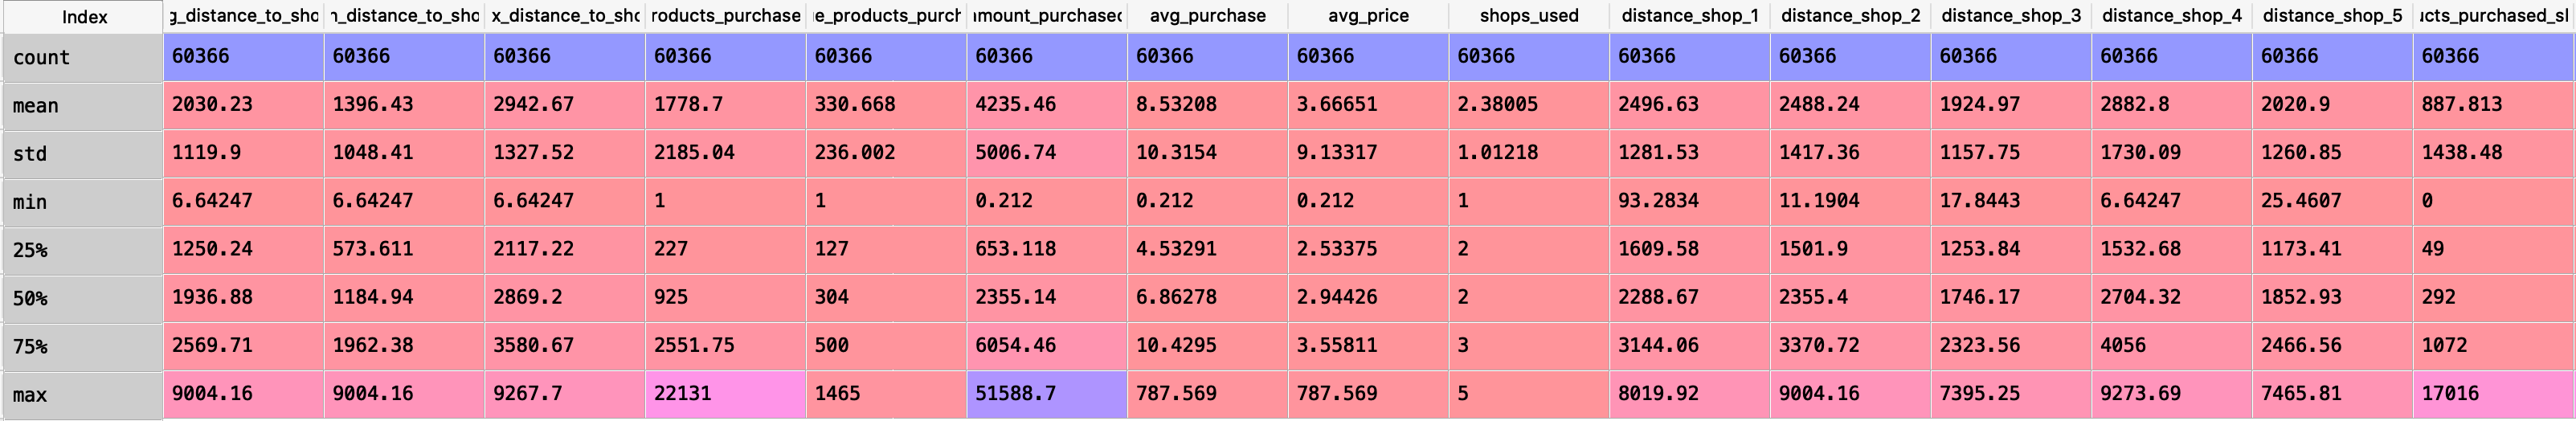
\includegraphics[scale=0.30]{summary.png}
\end{center}

\noindent
Nous voyons qu'il existe une seule variable qualitative, la variable 'shops used', les autres étant toutes des variables quantitatives continues. Nous remarquons aussi que toutes les variables quantitatives affichent de grandes dispersions. Par exemple, en regardant le nombre de produits achetés, nous voyons que certains clients achètent très peu, soit 1 seul article, tandis que d'autres achètent jusqu'à 22 131 articles, la moyenne étant 2 552.75. Ce type d'observation nous permettra de mieux interpréter les clusters proposés par les différentes versions des k-means.

\vspace{5 mm}
\noindent
Une Analyse en Composantes Principales (ACP) est implémentée afin de mieux regrouper et comprendre les variables quantitatives. Les 3 premières composantes principales expliquent moins de la moitié de l'inertie, soit 41.58\% de la variance expliquée.  Nous n'étudierons pas les résultats de l'ACP dans notre situation si ce n'est pour nous aider à mieux distinguer les clusters proposés par la méthode de kmeans++ semi supervisé, et mieux les associer aux variables du jeu de données.

\begin{center}
\captionof{figure}{ACP en 3 dimensions}
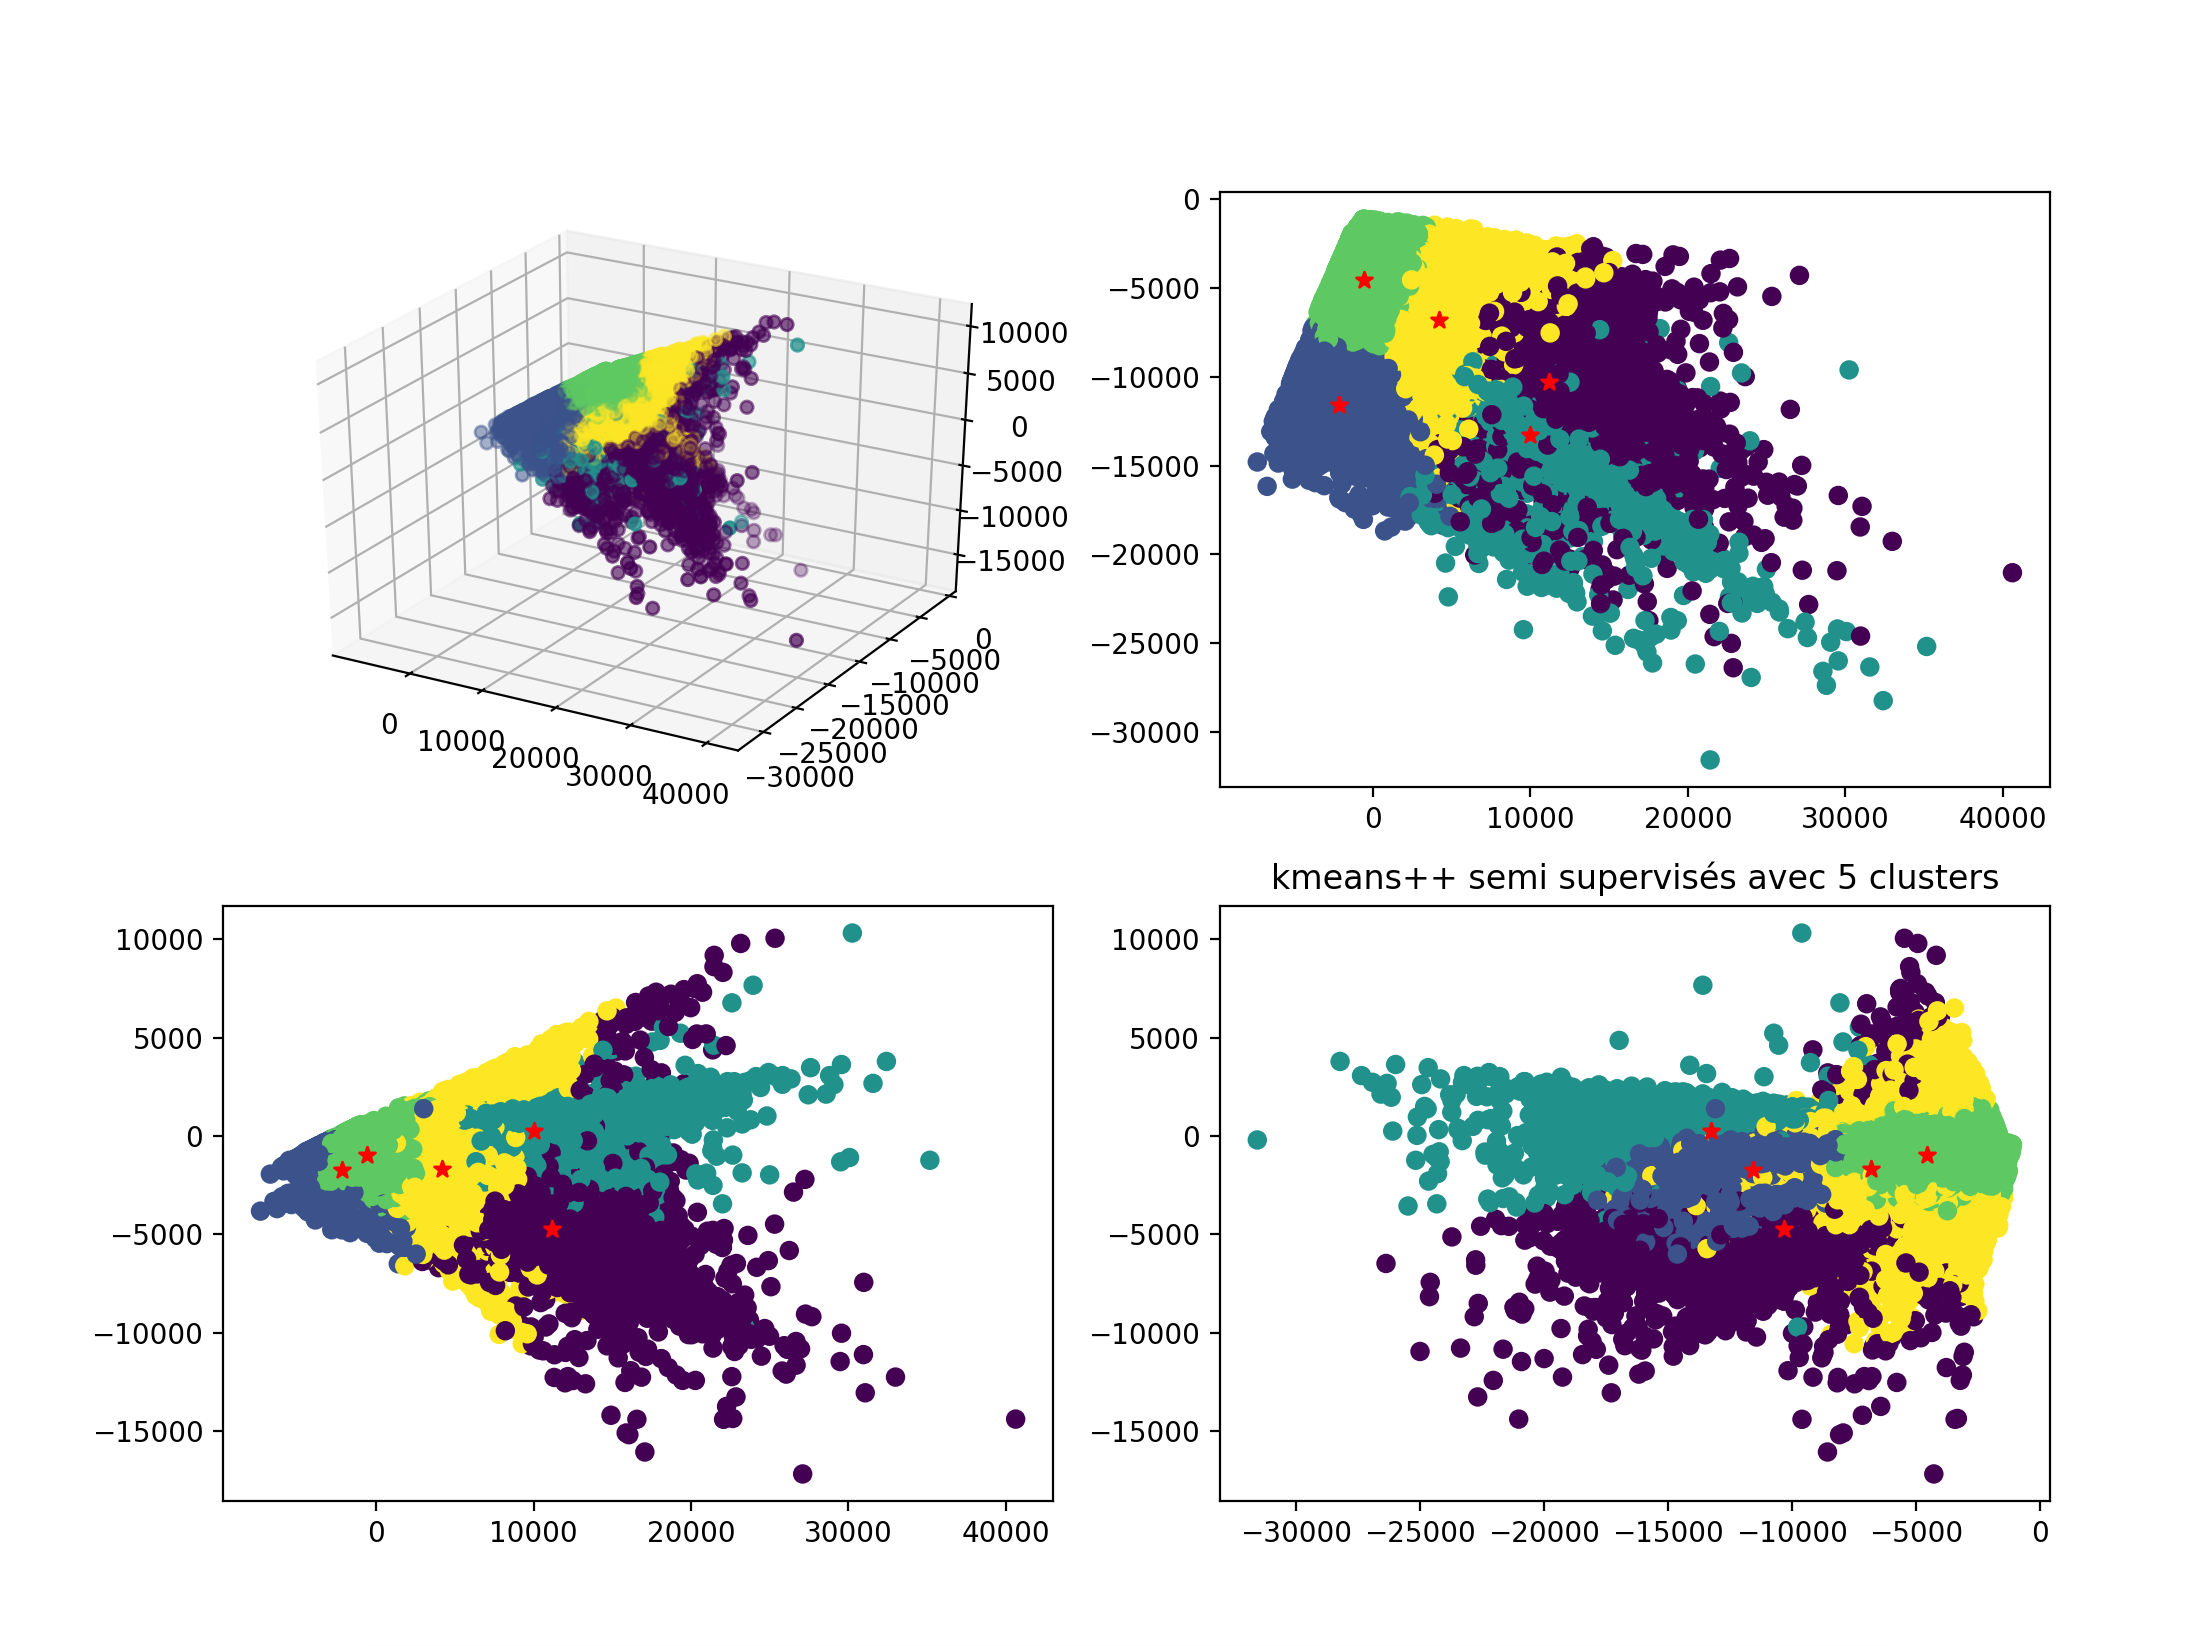
\includegraphics[scale=0.35]{ACP_3D.png}
\end{center}


\vspace{30 mm}
\noindent
\begin{large}
\subsection{Choix du nombre de clusters}
\end{large}
\vspace{5 mm}

\noindent
La méthode kmeans est une méthode d'apprentissage non-supervisée. Lors de son application les données sont séparées en plusieurs classes dont le nombre est prédéfini de façon à regrouper les individus ayant le plus de similarité. C'est ainsi qu'une des tâches clefs est de trouver le nombre approprié de classes, $k$. Il existe plusieurs techniques pour déterminer le nombre de classes. Nous discuterons que des cas les plus connus : 
\vspace{5 mm}
\begin{description}
  \item \textbf{1.} \textbf{Méthode du pouce:}
  
  Cette méthode est une méthode approximative où le nombre de classes, $k$ est déterminé par : 
$ k \approx \sqrt{n/2}$

\vspace{5 mm}
    \item \textbf{2. L'indice de qualité}:
    
	Afin d'évaluer la qualité de la classification, les indices inertiels (l’inertie intra-classes et l’inertie inter-classes) sont souvent utilisés. L'inertie intra-classes ‘mesure le degré d’homogénéité entre les objets appartenant à la même classe' tandis que l’inertie inter-classes ‘mesure le degré d’hétérogénéité entre les classes.’
Il existe plusieurs indices de qualité, par exemple l’indice de Dunn, l’indice de Calinski et Harabasz (CH) ou encore l’indice de Silhouette. 
Le premier calcule la distance minimale inter-classes et ainsi plus cette distance est grande, meilleur sera la classification. 

\vspace{5 mm}
Introduit par Kauffman et Rousseew, l’indice de Silhouette nous donne une représentation visuelle de la distance entre un point d’une classe avec les points des classes voisines. Plus le coefficient ainsi calculé est proche de 1, plus la distance avec les classes voisines (inertie inter) est grande. Ceci s'observe notamment pour le nombre de classes optimal. À l'inverse, un coefficient proche de -1 nous indique une mauvaise classification de l’observation.

\vspace{5 mm}
		\item \textbf{3. Méthode du coude}:
		
  La méthode du coude est une technique visuelle très connue. L’idée derrière cette technique est d’implémenter la méthode K-means en parcourant k valeurs. À chacune des k valeurs, la somme des erreurs au carré est calculée et est affichée sur un graphique, nous permettant de mieux visualiser les résultats. L’objectif est de choisir la valeur k (qui sera le nombre de classes) créant un effet de ‘coude’, c’est-à-dire provoquant une baisse plus conséquente, plus soudaine de la somme des erreurs au carré. Nous disons ceci en gardant en tête que la somme des erreurs aura toujours tendance à baisser, plus la valeur de k est grande. 

\vspace{5 mm}
 	 \item \textbf{4. La validation croisée}:
 	 
La validation croisée regarde la stabilité des classes. Les données sont séparées en au moins deux parties. La première est utilisée pour former les classes tandis que la deuxième sert de validation. Lorsque nous parlons de stabilité, nous parlons de la fréquence à laquelle des classes similaires sont formées lorsque plusieurs itérations sont effectuées. Ainsi une plus grosse fréquence de l’apparition de mêmes classes équivaut à une plus grosse stabilité de ces classes.
 	 
\end{description}

\vspace{10 mm}
\noindent
Dans le cadre de notre étude, nous choisissons de travailler avec la méthode du coude, une méthode que nous appliquons sur la méthode de kmeans++ semi-supervisé avec 60\% de données labellisées. Cette méthode est d'ailleurs comparée avec celle de sklearn afin de déterminer l'exactitude de l'algorithme utilisé. Figure 3 affiche la répartition des sommes des erreurs au carré à la fois pour notre méthode, dite la méthode manuelle, ainsi que la méthode proposée par sklearn. Nous voyons une baisse plus soudaine lorsque nous avons 5 clusters. Ce sera ainsi le choix du nombre de clusters utilisé lors de l'application des algorithmes de clustering.

\begin{center}
\captionof{figure}{Méthode du coude, comparaison sklearn et méthode manuelle}
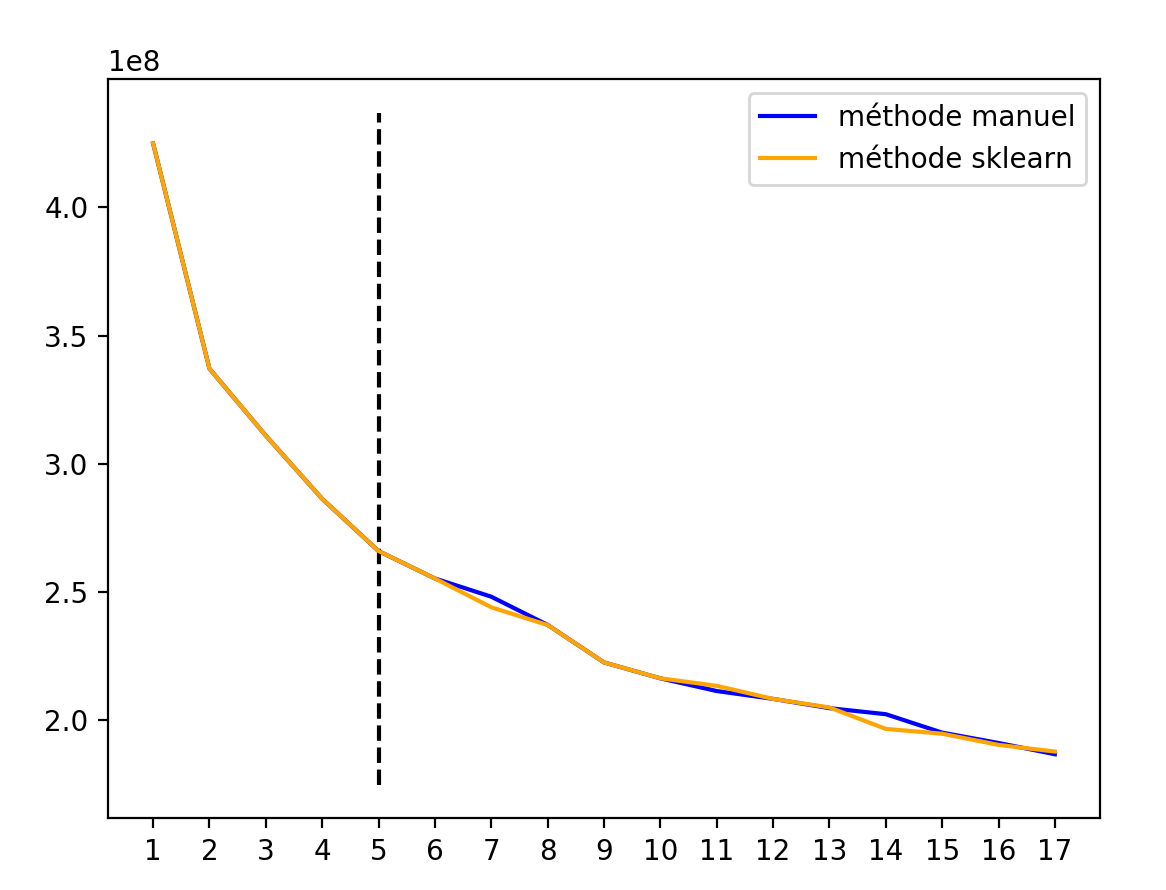
\includegraphics[scale=0.40]{elbow_final.png}
\end{center}

\vspace{10 mm}
\noindent
\begin{large}
\subsection{Résultats des expérimentations}
\end{large}
\vspace{10 mm}

\noindent
Dans cette section nous cherchons à présenter les résultats obtenus par les algorithmes kmeans, kmeans++ et kmeans++ semi supervisés. De plus ce dernier a été analysé plus en détails afin d'afficher l'impact des différents pourcentages de données labellisées. Comme pour l'ACP la variable qualitative a été écartée de notre analyse.
6 essais ont été effectués afin d'évaluer le temps d'exécution des algorithmes (en secondes). La moyenne des distances intra-classes a été obtenue en se basant sur 100 simulations. Le nombre de clusters, déterminé en utilisant la méthode du coude, est 5. Nous baserons le reste de notre étude sur ces 5 clusters.

\noindent
Nous cherchons en premier lieu à comparer les résultats de différents algorithmes. Les tableaux ci-dessous les affichent.

\begin{table}[ht]

\vspace{5 mm}

\begin{center}
\caption{\textbf{Résultats en utilisant kmeans}} 
\end{center}

\begin{adjustbox}{width=\columnwidth,center}
\begin{tabular}{c|c|c|c}
\hline
\rowcolor{Gray}

Temps d'exécution Minimum & Temps d'exécution Maximum & Temps d'exécution Moyen & Moyenne des distances intra-classe \\
\hline
0.867459&4.278867& 1.867284& \cellcolor{LightCyan}267024131.97\\

\end{tabular}
\end{adjustbox}



\vspace{5 mm}

\begin{center}
\caption{\textbf{Résultats en utilisant kmeans++}} 
\end{center}

\begin{adjustbox}{width=\columnwidth,center}
\begin{tabular}[scale=0.50]{c|c|c|c}
\hline
\rowcolor{Gray}
Temps d'exécution Minimum & Temps d'exécution Maximum & Temps d'exécution Moyen & Moyenne des distances intra-classe \\
\hline
0.952380&1.963426& 1.603216& \cellcolor{LightCyan}269311160.94\\

\end{tabular}
\end{adjustbox}


\vspace{5 mm}

\begin{center}
\caption{\textbf{Résultats en utilisant kmeans++ semi-supervisées avec 60\% de données labellisées}} 
\end{center}

\begin{adjustbox}{width=\columnwidth,center}
\begin{tabular}{c|c|c|c}
\hline
\rowcolor{Gray}
Temps d'exécution Minimum & Temps d'exécution Maximum & Temps d'exécution Moyen & Moyenne des distances intra-classe \\
\hline
0.386259&0.616933& 0.481936& \cellcolor{LightCyan}265971783.28\\
\end{tabular}
\end{adjustbox}


\end{table}

\vspace{20 mm}

\noindent 
Tel qu'attendu la durée d'exécution moyenne de l'algorithme de kmeans est plus longue que celle du kmeans++ et du kmeans++ semi-supervisée (avec 60\% de données labellisées). Cette dernière est d'ailleurs en moyenne 3 fois plus rapide que le kmeans ou le kmeans++. Au niveau du coût de la fonction nous voyons que le kmeans ++ semi supervisée affiche à nouveau le meilleur résultat (avec la plus petite distance moyenne intra-classes sur 100 simulations). 

\vspace{5 mm}
\noindent 
Nous notons toutefois que la distance intra-classe moyenne lorsque kmeans est utilisé est plus petite que celle du kmeans++.  Bien qu'on se serait attendu à obtenir le résultat inverse, cette observation peut être due au fait que le jeu de données en question soit bien adapté aux kmeans. Ainsi, la qualité de classification obtenue par les kmeans est aussi bonne que celle des kmeans++. Cependant, les kmeans++ restent bien meilleurs dans le sens où l'algorithme est plus rapide pour des classifications considérées équivalentes.


\vspace{10mm}


\begin{table}[ht]
\footnotesize

\caption{\textbf{Résultats en utilisant kmeans++ semi-supervisées avec 25\% de données labellisées}} 

\begin{adjustbox}{width=\columnwidth,center}
\begin{tabular}{c|c|c|c}
\hline
\rowcolor{Gray}
Temps d'exécution Minimum & Temps d'exécution Maximum & Temps d'exécution Moyen & Moyenne des distances intra-classe \\
\hline
0.534357&0.759242& 0.629477& \cellcolor{LightCyan}265972507.4\\

\end{tabular}
\end{adjustbox}


\vspace{10 mm}
\caption{\textbf{Résultats en utilisant kmeans++ semi-supervisées avec 99\% de données labellisées}} 

\begin{adjustbox}{width=\columnwidth,center}
\begin{tabular}{c|c|c|c}
\hline
\rowcolor{Gray}
Temps d'exécution Minimum & Temps d'exécution Maximum & Temps d'exécution Moyen & Moyenne des distances intra-classe \\
\hline
0.115119&0.288531& 0.232994& \cellcolor{LightCyan}265976831.1\\
\end{tabular}
\end{adjustbox}

\end{table}

\vspace{5 mm}
\noindent
À partir des tableaux 4 et 5, nous voyons que plus le pourcentage de données est labellisé, plus le temps d'exécution est rapide. Toutefois, nous ne pouvons pas dire autant des distances intra-classe moyenne. En effet lorsque les données sont labellisées à 99\% nous avons une inertie plus élevée que lors que les données sont moins labellisées. Une nouvelle fois la problématique pourrait venir du jeu de données, ou encore du fait que la supervision est en fait une pseudo-supervision car les vrais labels n'étaient pas disponibles. Ainsi cela expliquerait la variation des inerties moyennes. C'est pour cela que nous nous baserons davantage sur la durée d'exécution comme mesure de performance.
\vspace{20 mm}

\noindent
\textbf{Interprétation}


\vspace{5 mm}
\noindent
Nous cherchons désormais à interpréter les résultats obtenus sur le jeu de données utilisé dans cette étude. Figure 4 affiche les 5 clusters ainsi que leurs centres, tels que proposés par l'algorithme des kmeans++ semi-supervisés avec 60\% de données labellisées. Nous rappelons que le nombre de clusters a préalablement été choisi par la méthode du coude.
\vspace{10 mm}

\begin{center}
\captionof{figure}{Affichage 5 clusters et 5 centres, determiné par kmeans++ semi-supervisé}
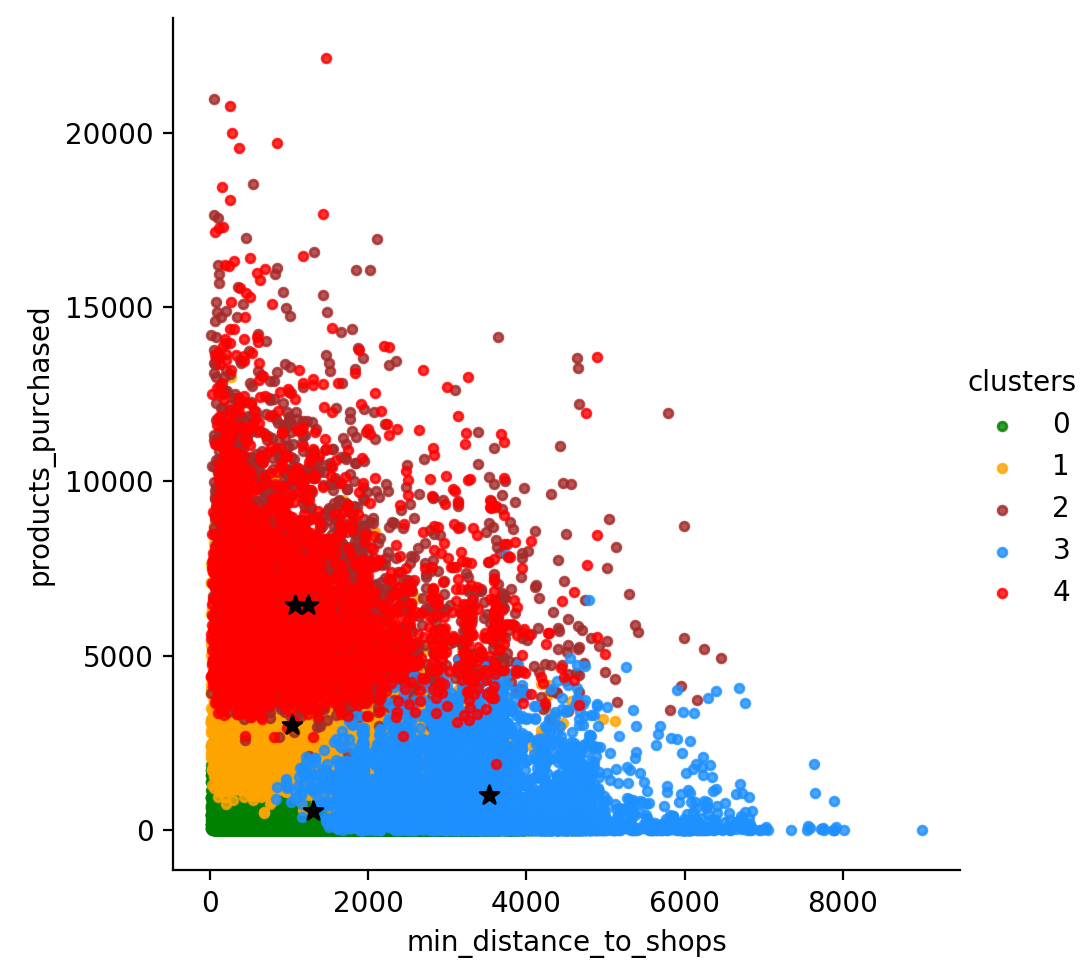
\includegraphics[scale=0.40]{kmeanspp_clusters.png}
\end{center}


\vspace{10 mm}
\noindent
Nous pouvons clairement voir que les clusters 1 et 3 (orange et rouge) sont moins distincts entre eux contrairement aux autres clusters. Effectivement, les centres de ces deux clusters sont très proches suggérant que nous aurions pu regrouper ces deux clusters. Nous avons choisi ici de représenter le nuage de points associé aux variables \verb|products_purchased| et \verb|min_distance_to_shops|. Ces variables ont été choisies car les clusters sont bien discriminés.  

\noindent
Ce que nous pouvons déduire du graphique est que les clients appartenant au cluster 4 sont ceux parcourant les plus petites distances par rapport aux magasins à l'inverse de ceux du cluster 0. D'ailleurs nous voyons que ces derniers achètent le moins de produits, tout comme les clients du cluster 2. Ainsi, nous pouvons établir un lien entre la distance parcourue pour aller au magasin et le nombre de produits achetés. En général, plus un client devra parcourir une plus longue distance, moins il ira au magasin, et le moins de produits il achètera. Sur un plan commercial et marketing, ce seront ainsi les clients des clusters 1,3 et 4 qui devraient être ciblés comme étant des acheteurs potentiels.


\vspace{5 mm}
\noindent
Nous cherchons désormais à établir d'autres liens avec les variables utilisées dans notre jeu de données. Nous commençons par analyser la variable qualitative \verb|shops_used|. Figure 5 nous affiche la répartition des magasins ciblés dans l'étude. Les magasins 4 et 5 semblent être les plus proches des clients. Pour le magasin 3 et le 4 (bien que la répartition du nuage de celui-ci est moins distinct que celui du magasin 3 sur le graphique), il est clair que moins le client voyage, plus il achète des produits. Toutefois vu la grande quantité de données, il est difficile de bien différencier les clusters, ainsi il faudra d'autres graphiques pour confirmer nos résultats.

\begin{center}
\captionof{figure}{Variable qualitative}
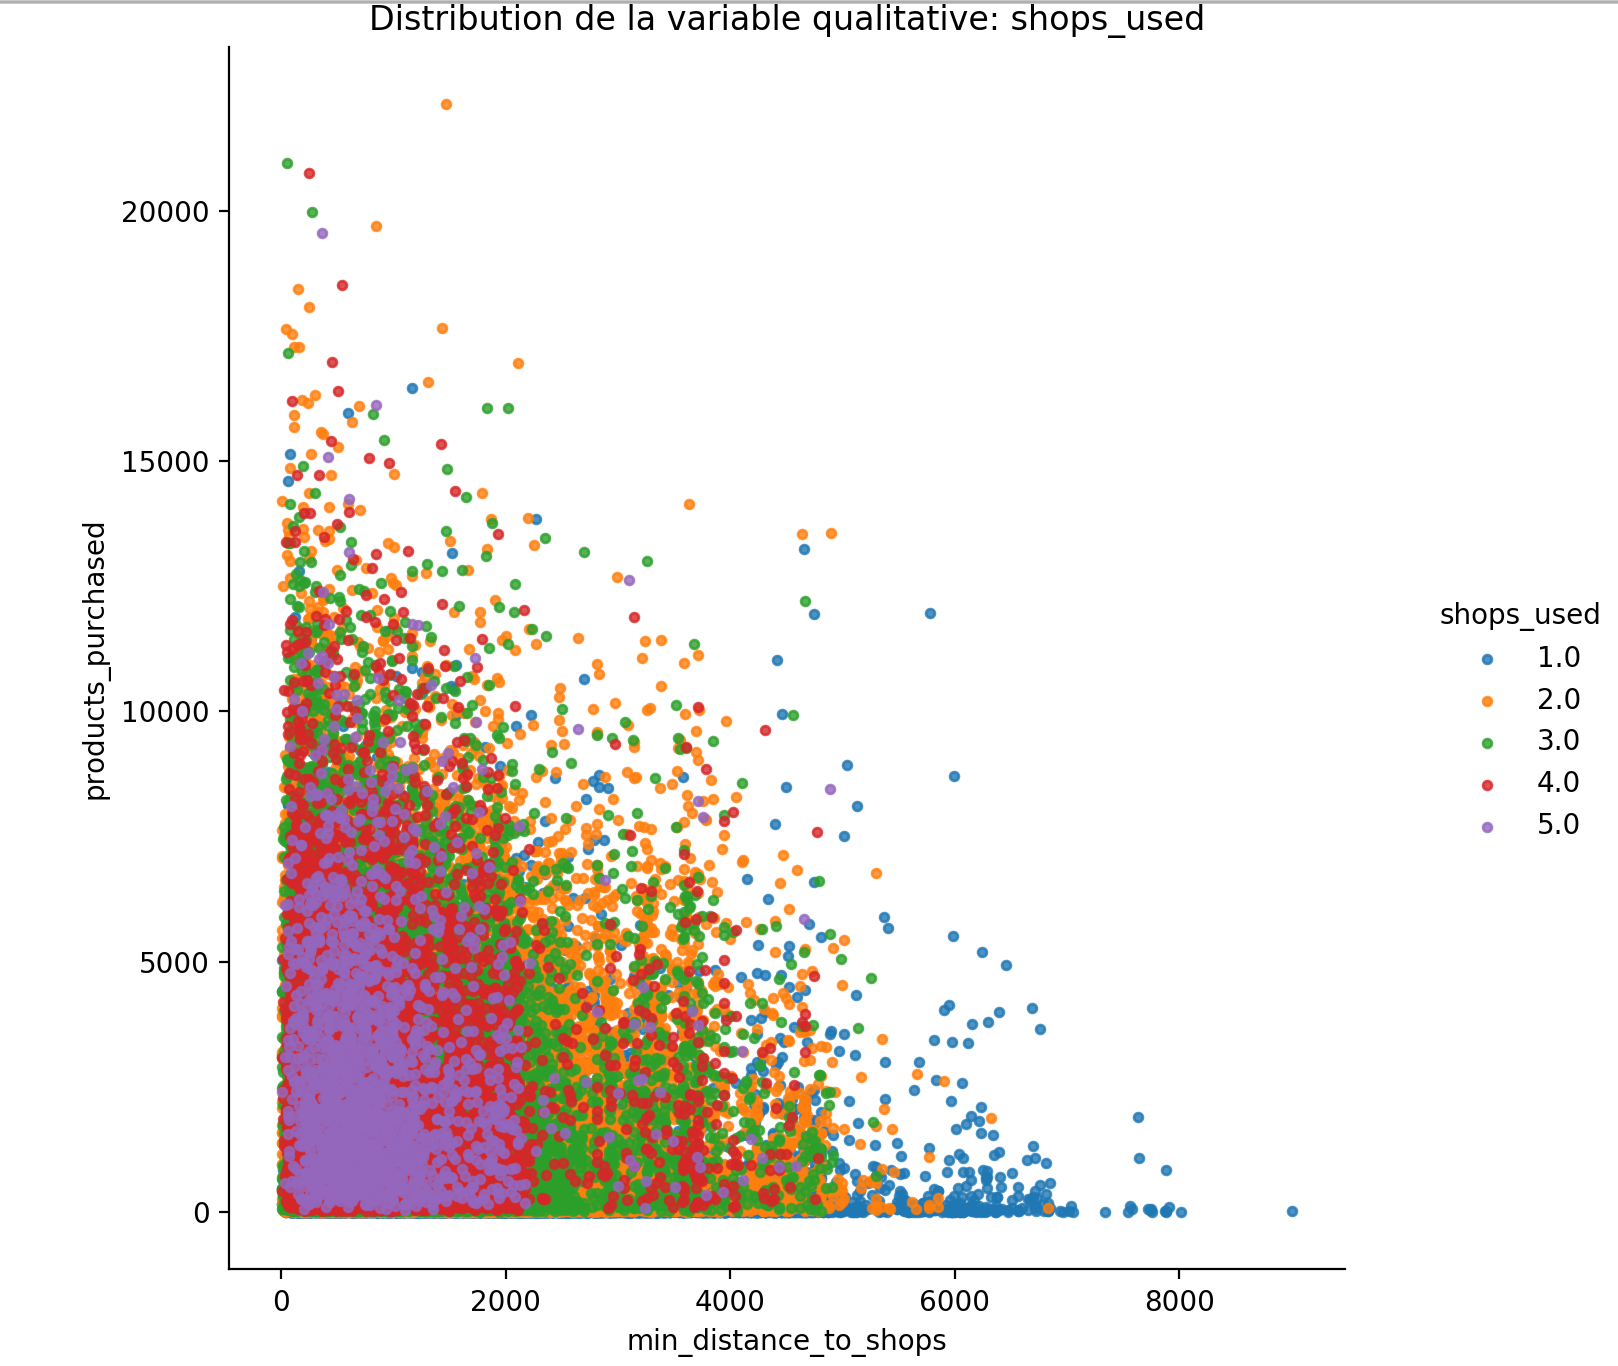
\includegraphics[scale=0.40] {shops_used.png}
\end{center}


\vspace{5 mm}
\noindent
Figure 6 ci-dessous affichent la relation entre la distance pour aller à chaque magasin et le nombre de produits achetés dans ces magasins. Nous voyons dans le  premier graphique que les clients des clusters 1, 2 et 3 semblent avoir une préférence pour le magasin 1. Les clients du cluster 5 sont ceux qui semblent habiter le plus loin du magasin 1. En revanche bien qu'ils en soient plus éloignés, leur consommation semble être un peu plus grande qu'au magasin 2, suggérant qu'ils préfèrent acheter les produits du magasin 1 au 2. Pour les 3 derniers graphiques, il est difficile d'établir un lien évident car les observations sont mélangées et peu distinguables. Nous nous baserons sur d'autres graphiques afin de tirer des conclusions.


\begin{center}
\captionof{figure}{Relation nombre de produits acheté et distance pour chaque magasin}
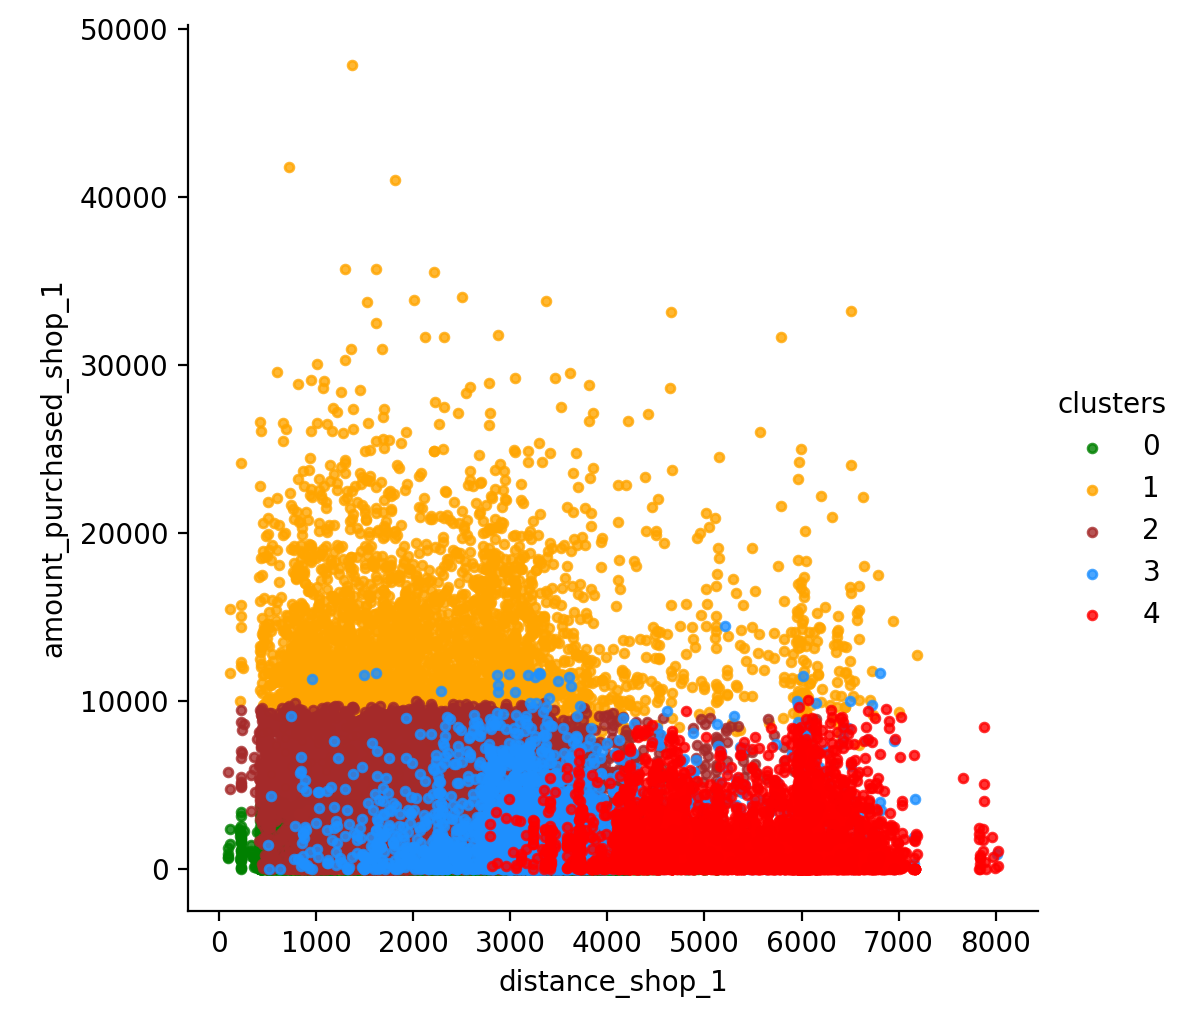
\includegraphics[scale=0.30] {shop1_amountpurchased.png}
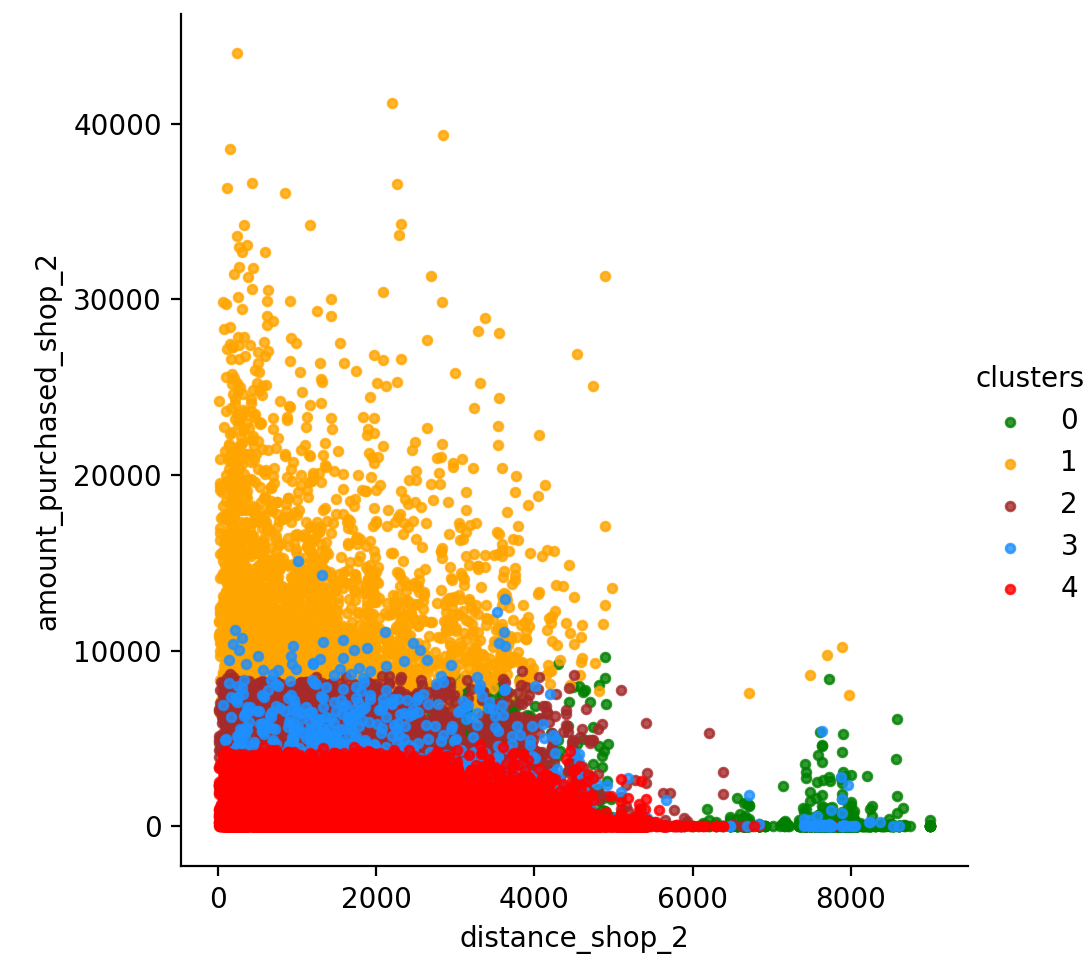
\includegraphics[scale=0.30] {shop2_amountpurchased.png}
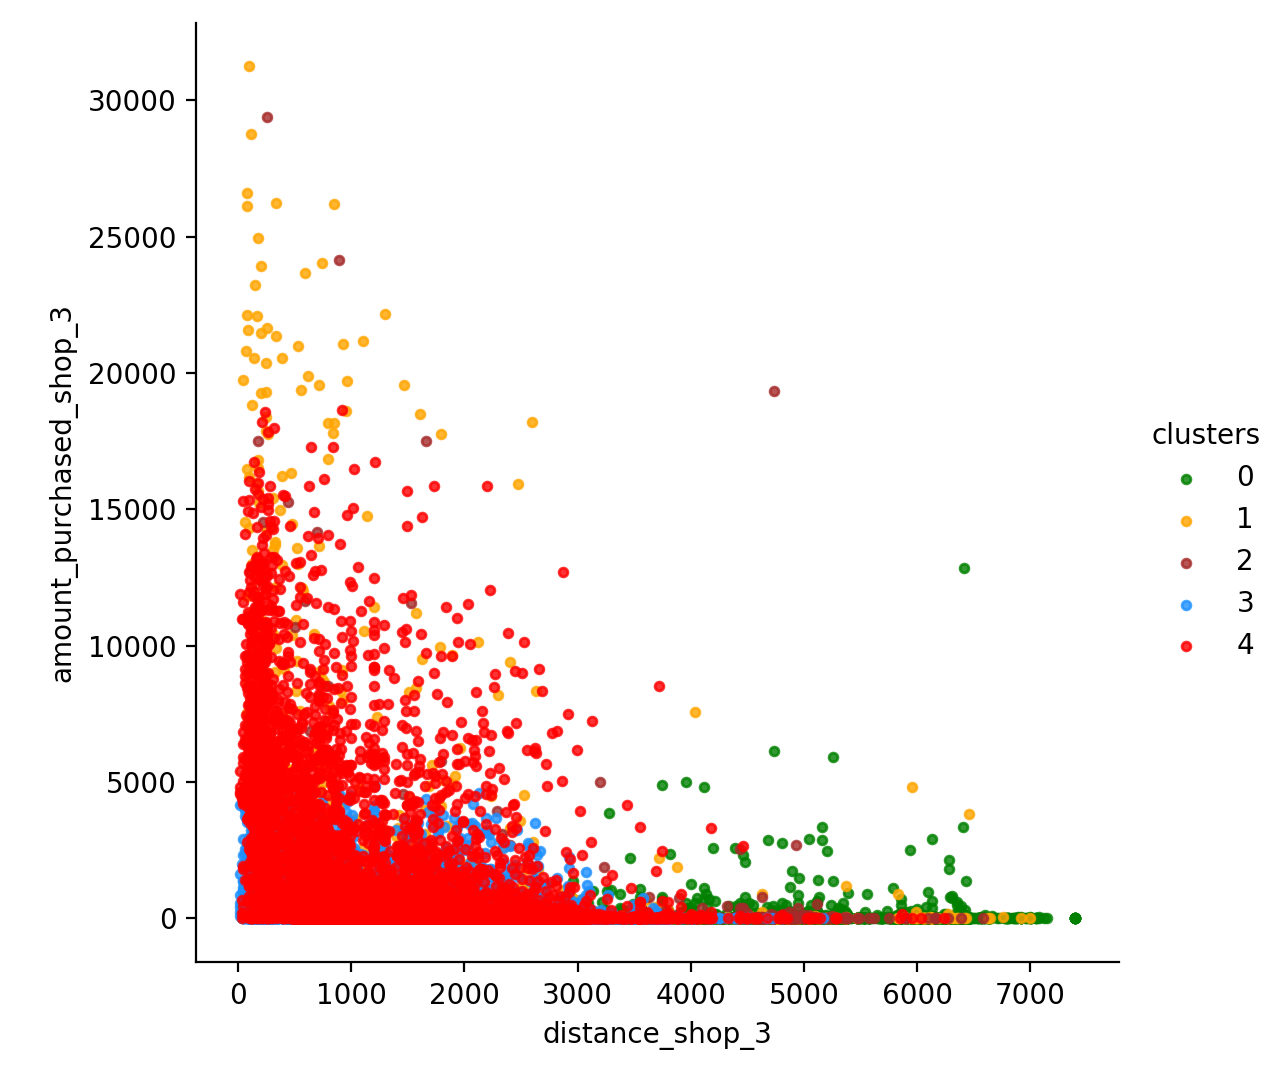
\includegraphics[scale=0.30] {shop3_amountpurchased.png}
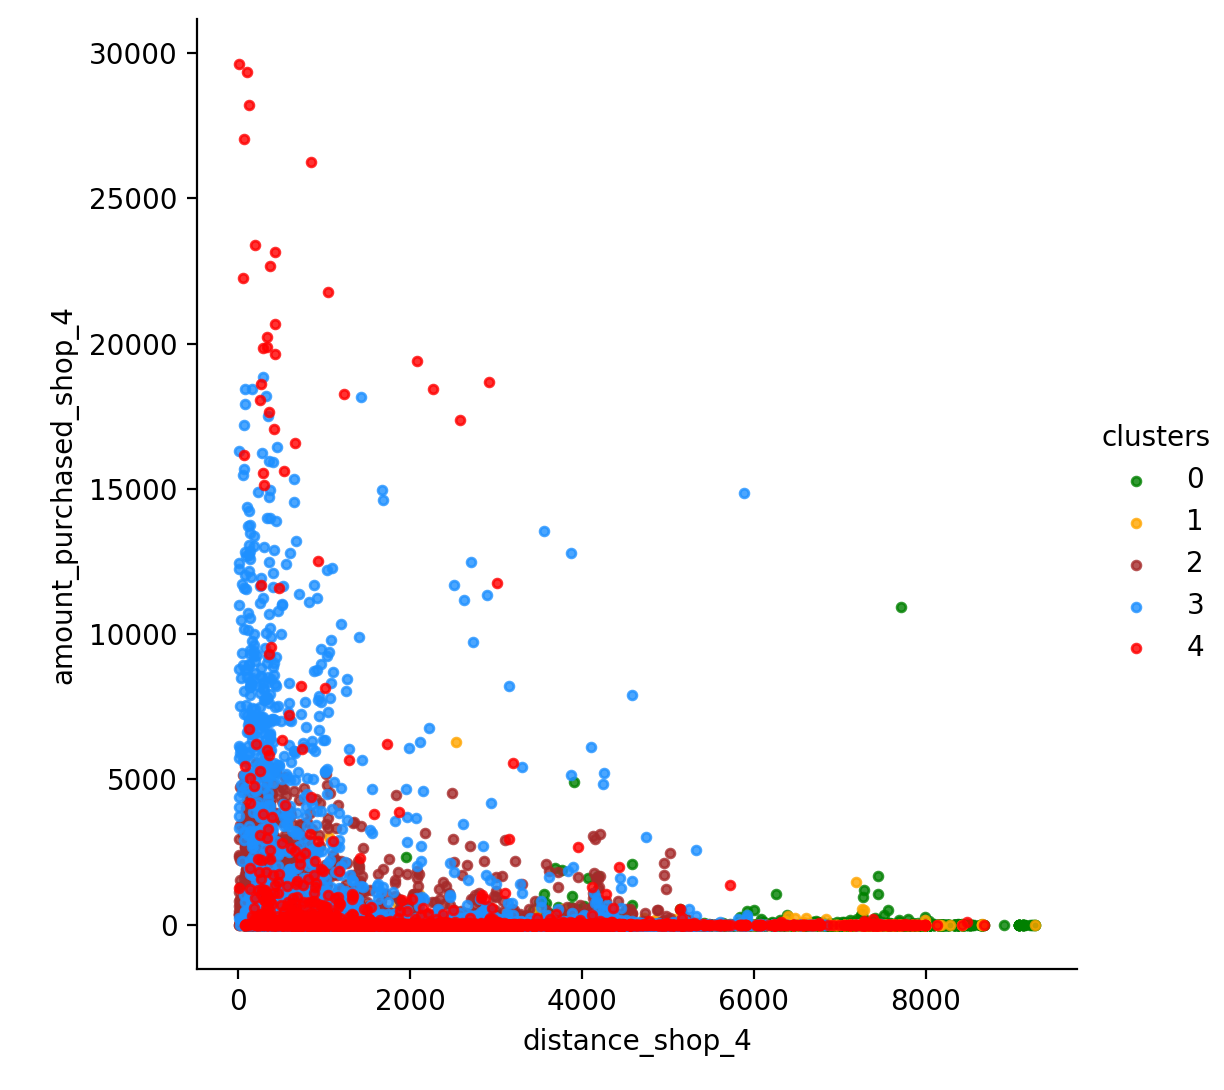
\includegraphics[scale=0.30] {shop4_amountpurchased.png}
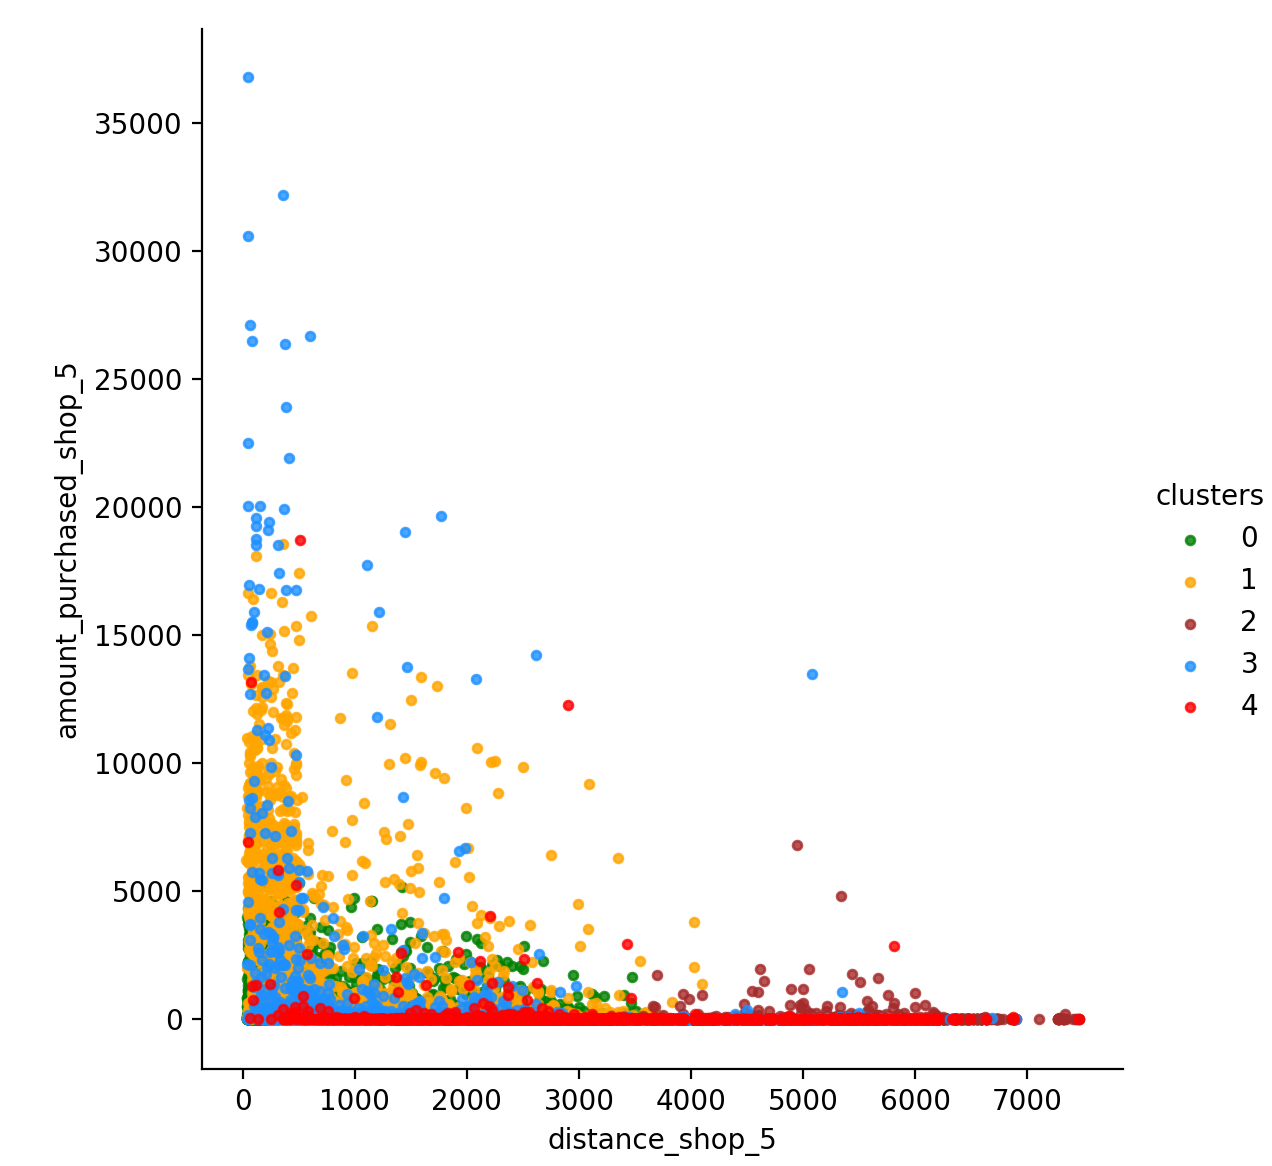
\includegraphics[scale=0.30] {shop5_amountpurchased.png}
\end{center}


\noindent
Nous utilisons des diagrammes en barre (voir ci-dessous) afin de nous aider à mieux comprendre le nombre de clients allant dans les magasins ainsi que les quantités exactes de produits vendus. Nous voyons que le magasin 5 est celui qui vend le plus de produits (unique et globalement) et c'est celui qui affiche le plus petit prix moyen des produits. Ainsi, les magasins 5 et 4 sont les magasins les plus vendeurs. Le magasin 1 est celui qui vend les produits les plus chers. Il n'est donc pas étonnant de voir qu'il vend une plus petite quantité de produits. Finalement, nous voyons quand même que plus de clients vont aux magasins 1 et 2, le magasin 5 étant celui qui a le moins de clients. De ces observations nous comprenons que les magasins 1 et 2 sont des magasins qui vendent des produits plus chers, avec pour conséquence le fait que même si les clients y vont plus souvent, ils ne vont pas nécessairement acheter les produits de ces magasins. 


\noindent
\begin{center}
\captionof{figure}{Diagrammes de barre affichant le prix moyen, nombre de produits vendus et nombre clients allant dans chaque magasin }
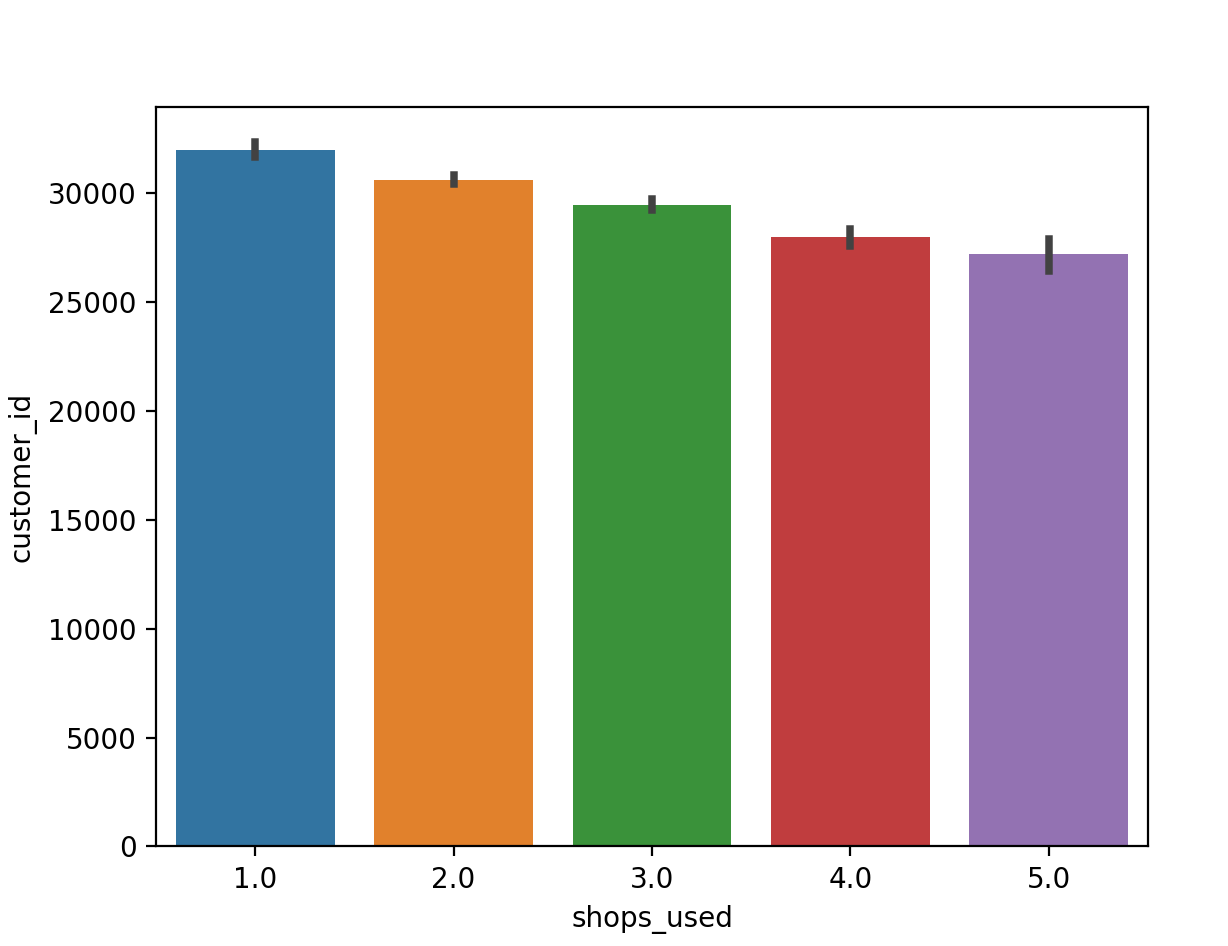
\includegraphics[scale=0.30] {clients_shops.png}
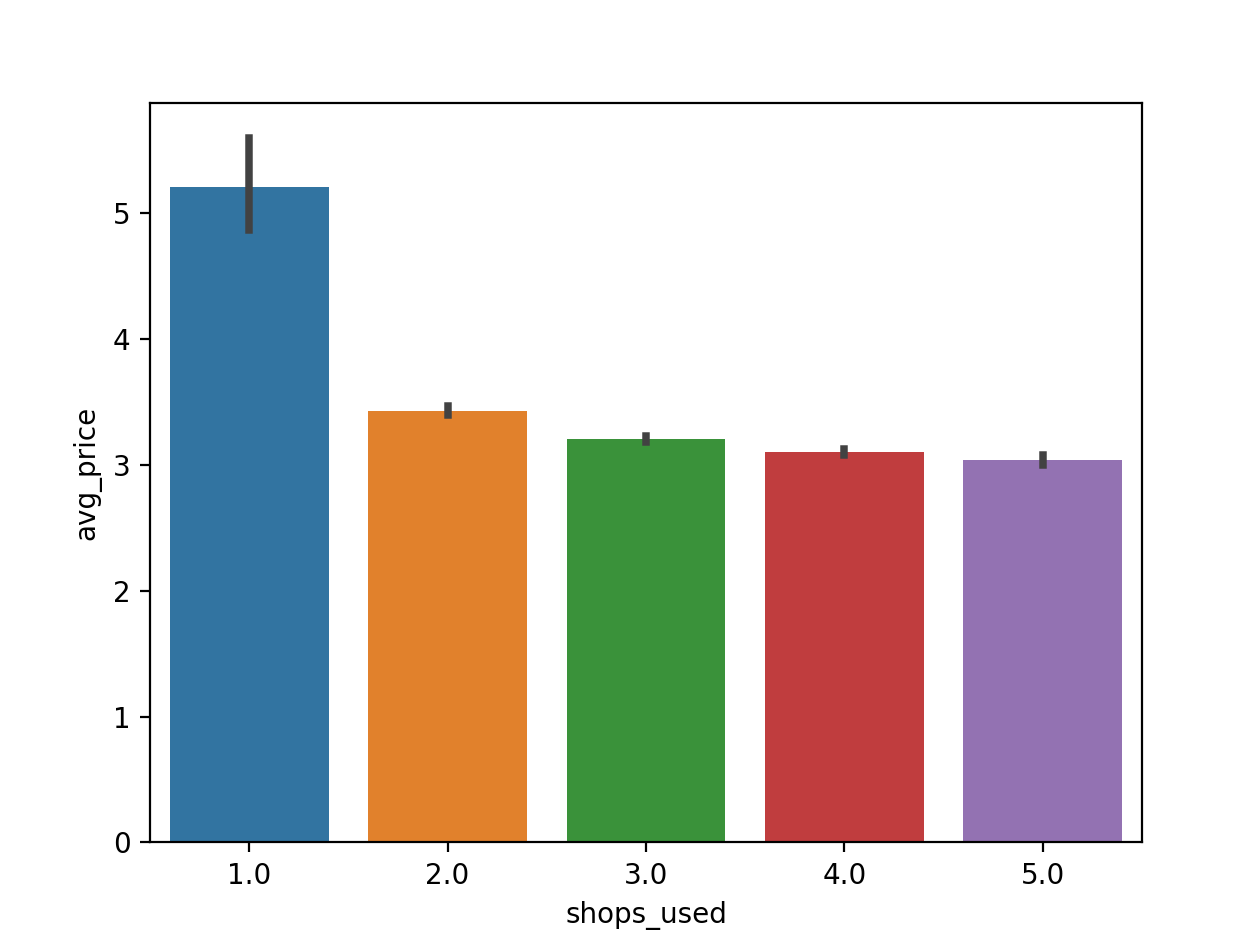
\includegraphics[scale=0.30] {price_shops.png}
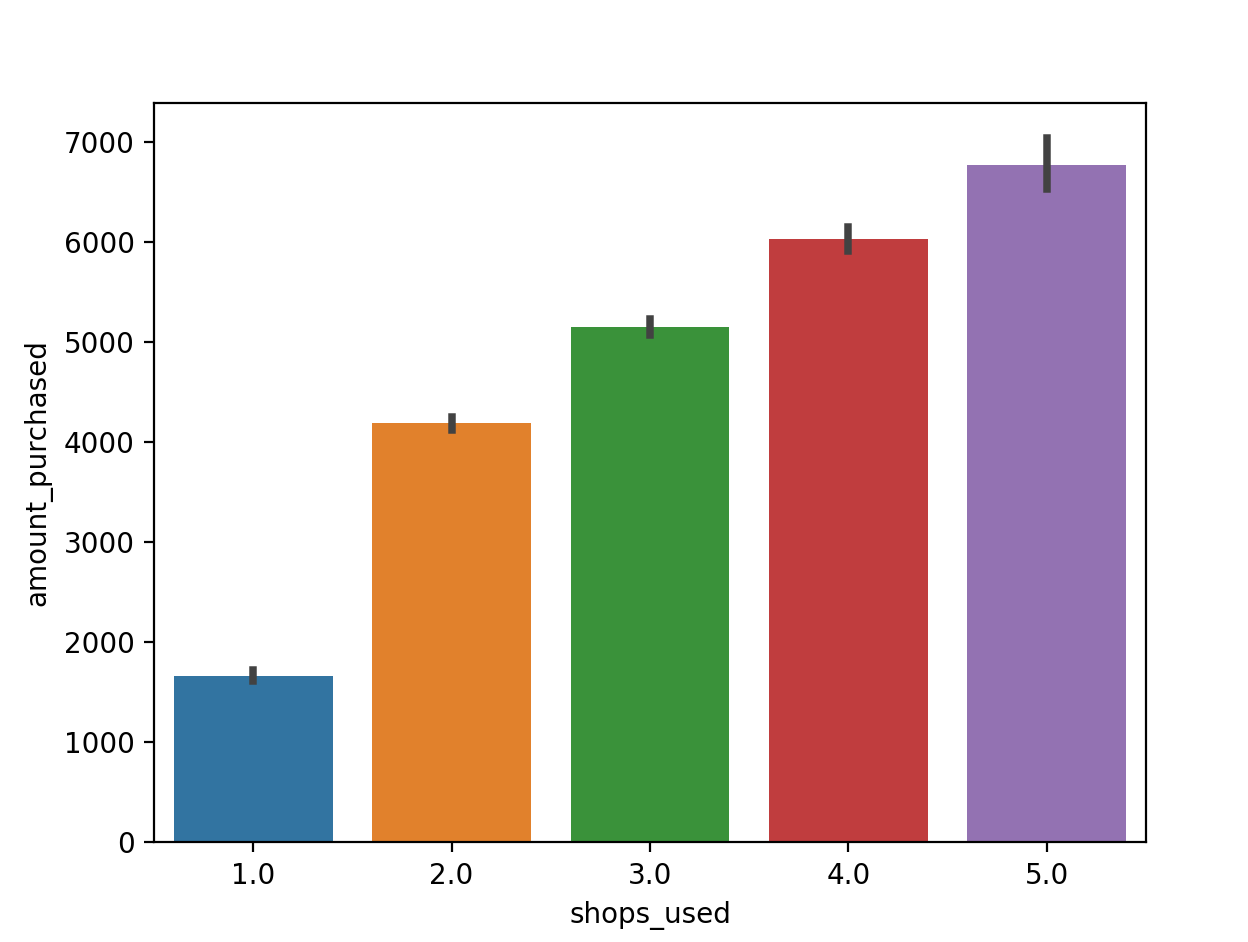
\includegraphics[scale=0.30] {amountpurchased_shops.png}
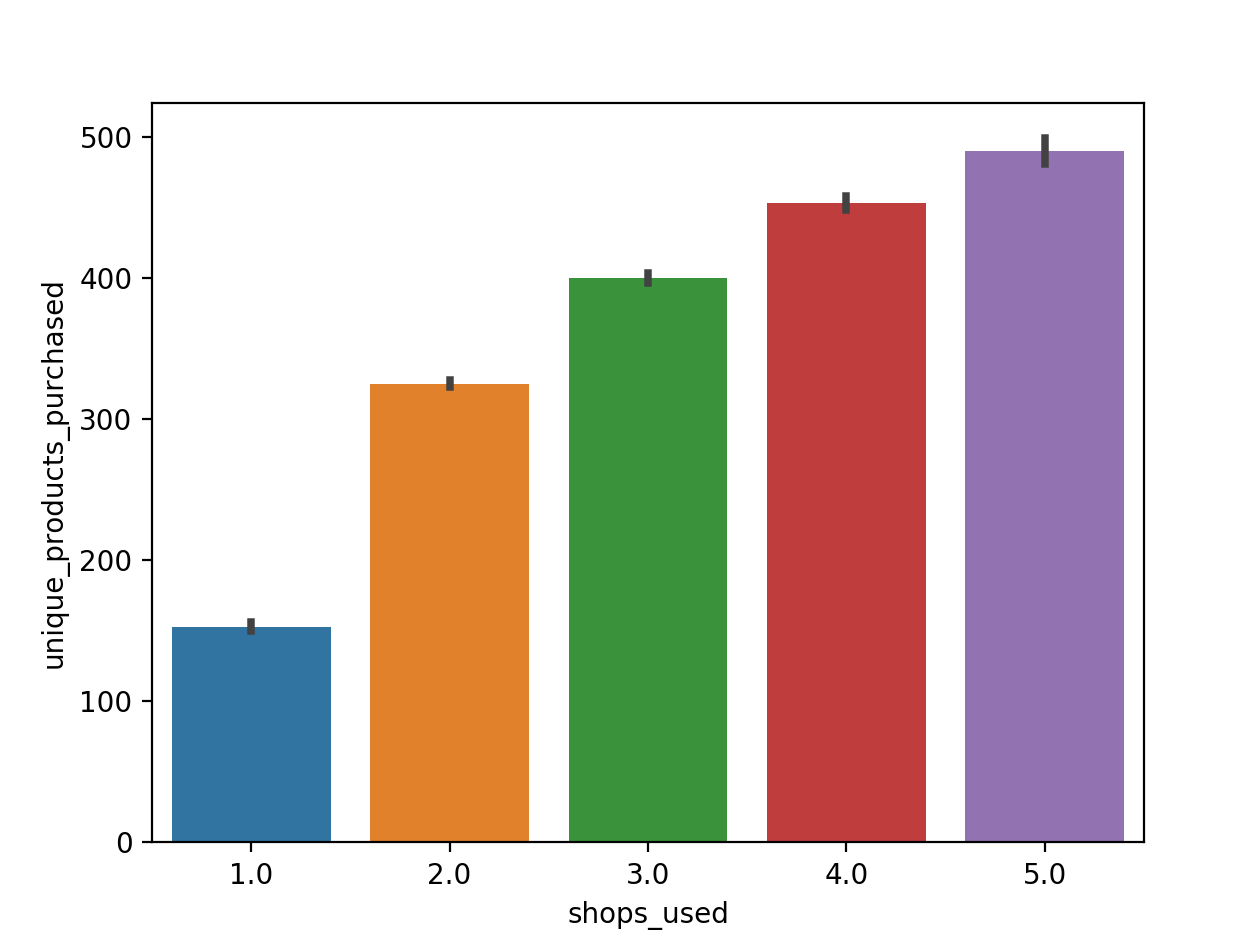
\includegraphics[scale=0.30] {unique_shops.png}
\end{center}

\noindent
Toutes ces observations nous poussent à dire que la consommation diminue lorsque les prix augmentent, et ainsi les magasins les moins chers, soit 4 et 5, sont ceux vendant le plus de produits. Ils ont également plus de produits uniques que les magasins plus chers comme les 1 et 2. Ces derniers attirent beaucoup de clients, mais ceux-ci n'achèteront pas nécessairement les produits, d'où le fait que ces types de magasins vendent moins de produits. Au niveau des marges d'affaires de ces magasins, nous voyons dans le diagramme ci-dessous qu'il n'y a pas de grande différence entre ces boutiques. Effectivement, le quantité de consommation est compensée par le prix, ce qui fait que la vente moyenne reste plus ou moins égale.

\vspace{5 mm}
\begin{center}
\captionof{figure}{Nombre moyen de produits vendus par chaque magasin}
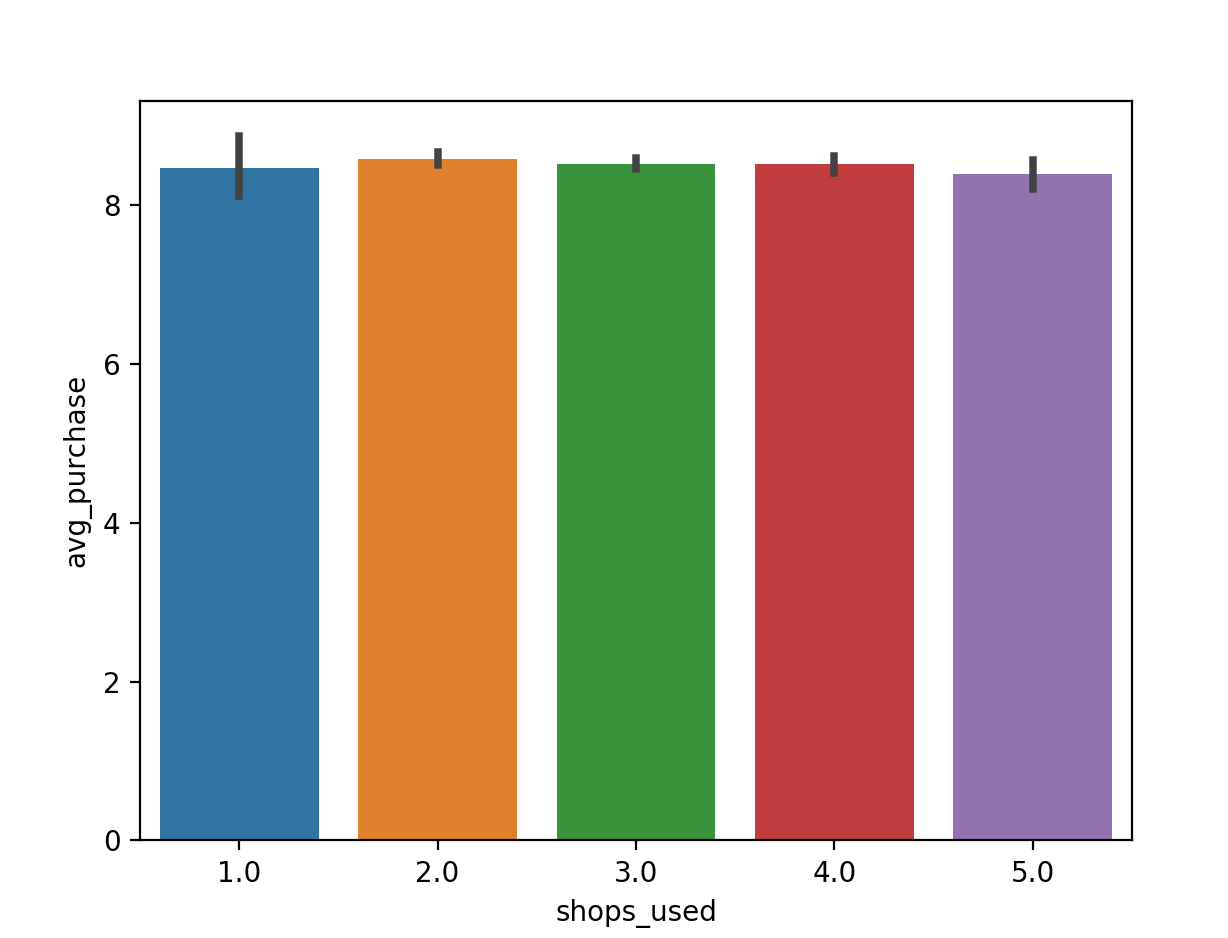
\includegraphics[scale=0.30] {avgpurchased_shops.png}
\end{center}

\noindent
Nous cherchons maintenant à lier ces observations aux clusters obtenus par les kmeans++ semi-supervisés. Pour cela nous utilisons à nouveau des diagrammes en barre qui affichent le nombre d'individus de clusters qui achètent dans les différents magasins. À l'aide de ces graphiques (Figure 9), nous pouvons établir que certains magasins attirent davantage certains clients.

\vspace{5 mm}
\noindent
Le magasin 1 attire les individus du cluster 3, tandis que le magasin 2 attire plus le cluster 2, le magasin 3 attire les individus des clusters 1 et 2, le magasin 4 quant à lui attire les clients des clusters 2 et 3, et finalement le magasin 5 attire principalement les individus des clusters 4 et 3. Dans tous les cas le cluster 0 est celui qui est le moins représenté, confirmant le fait que ce cluster pourrait facilement être regroupé avec un autre cluster.\\ 


\begin{center}
\captionof{figure}{Nombre de produits achetés par chaque cluster, pour chaque magasin}
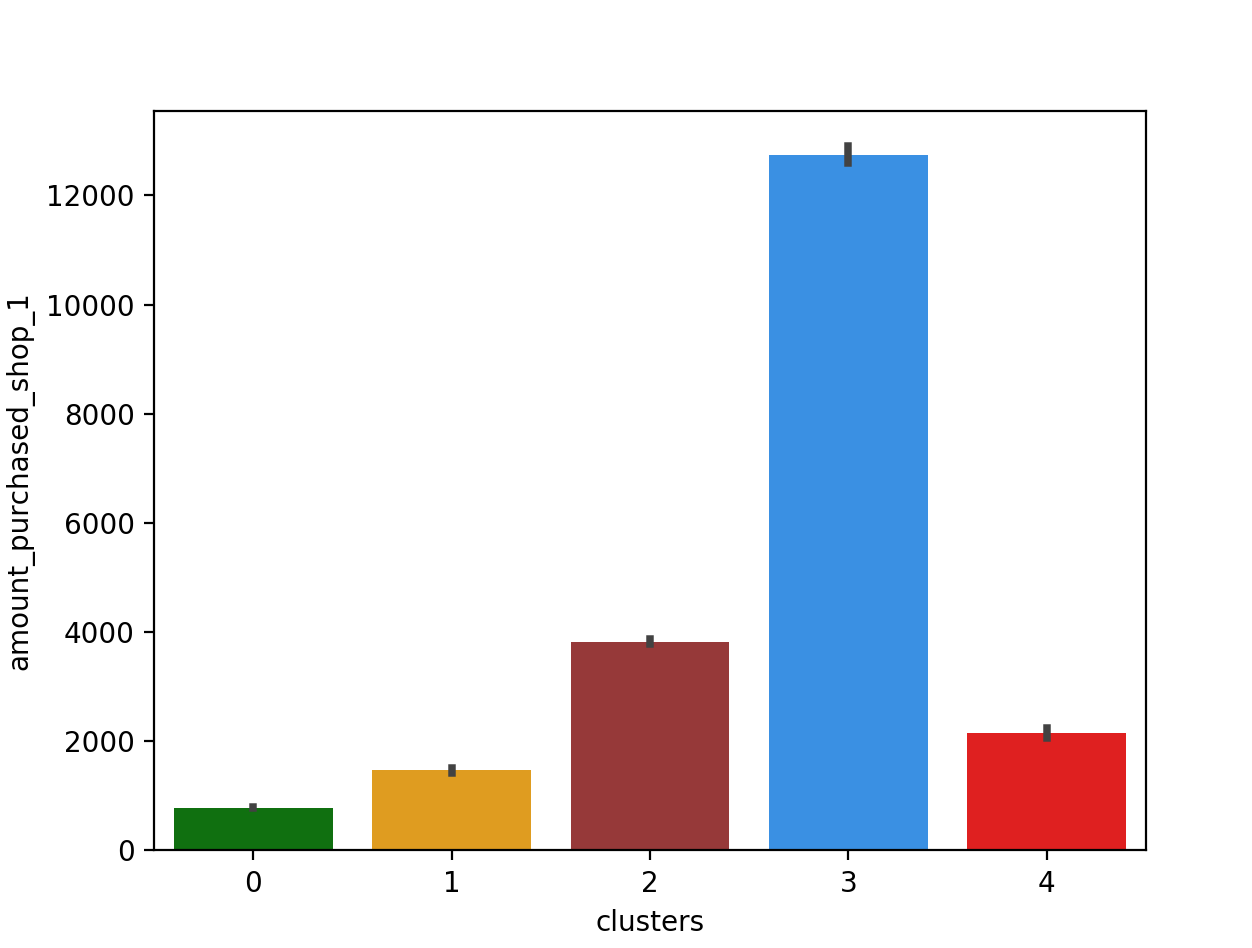
\includegraphics[scale=0.20] {cluster_shop1.png}
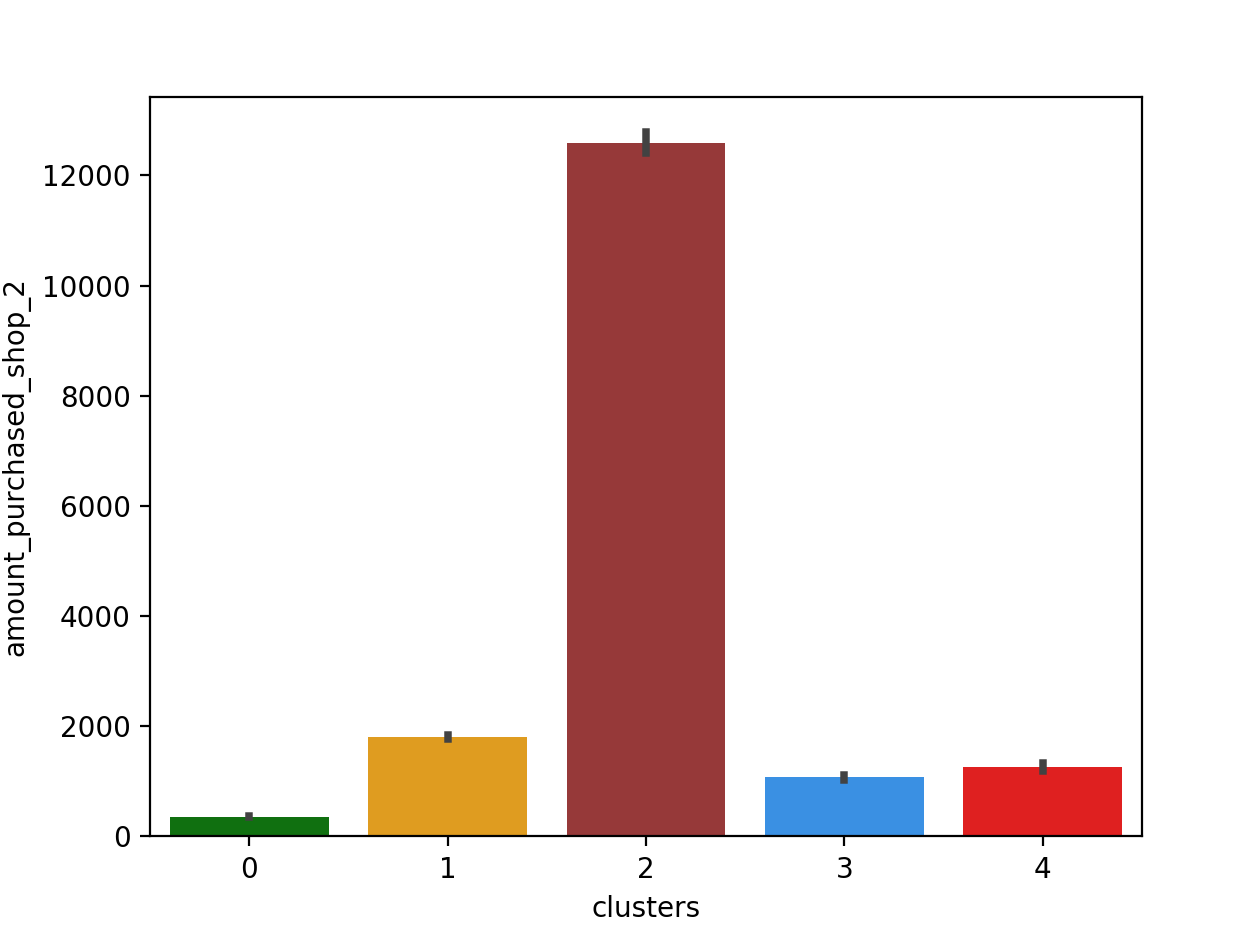
\includegraphics[scale=0.20] {cluster_shop2.png}
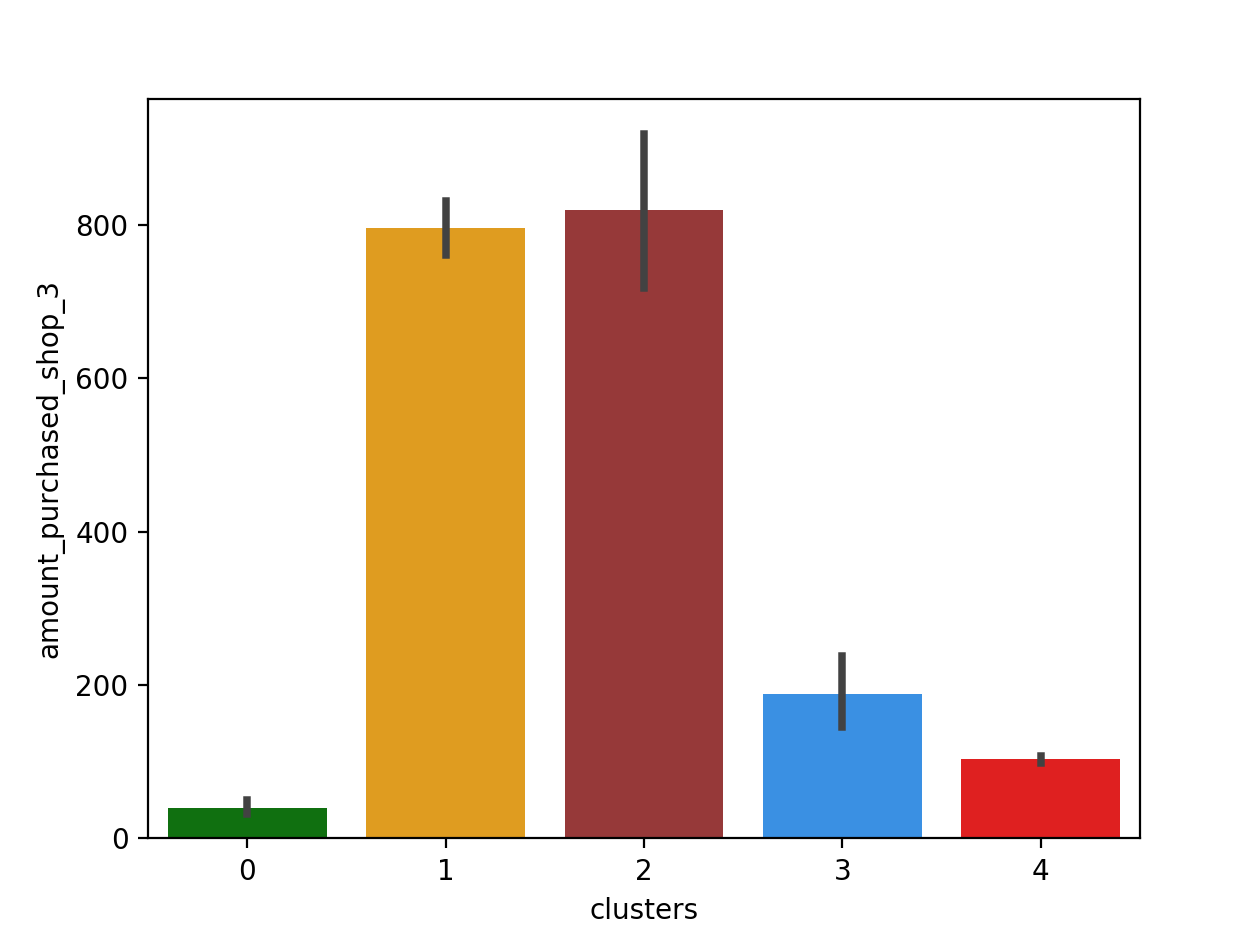
\includegraphics[scale=0.20] {cluster_shop3.png}
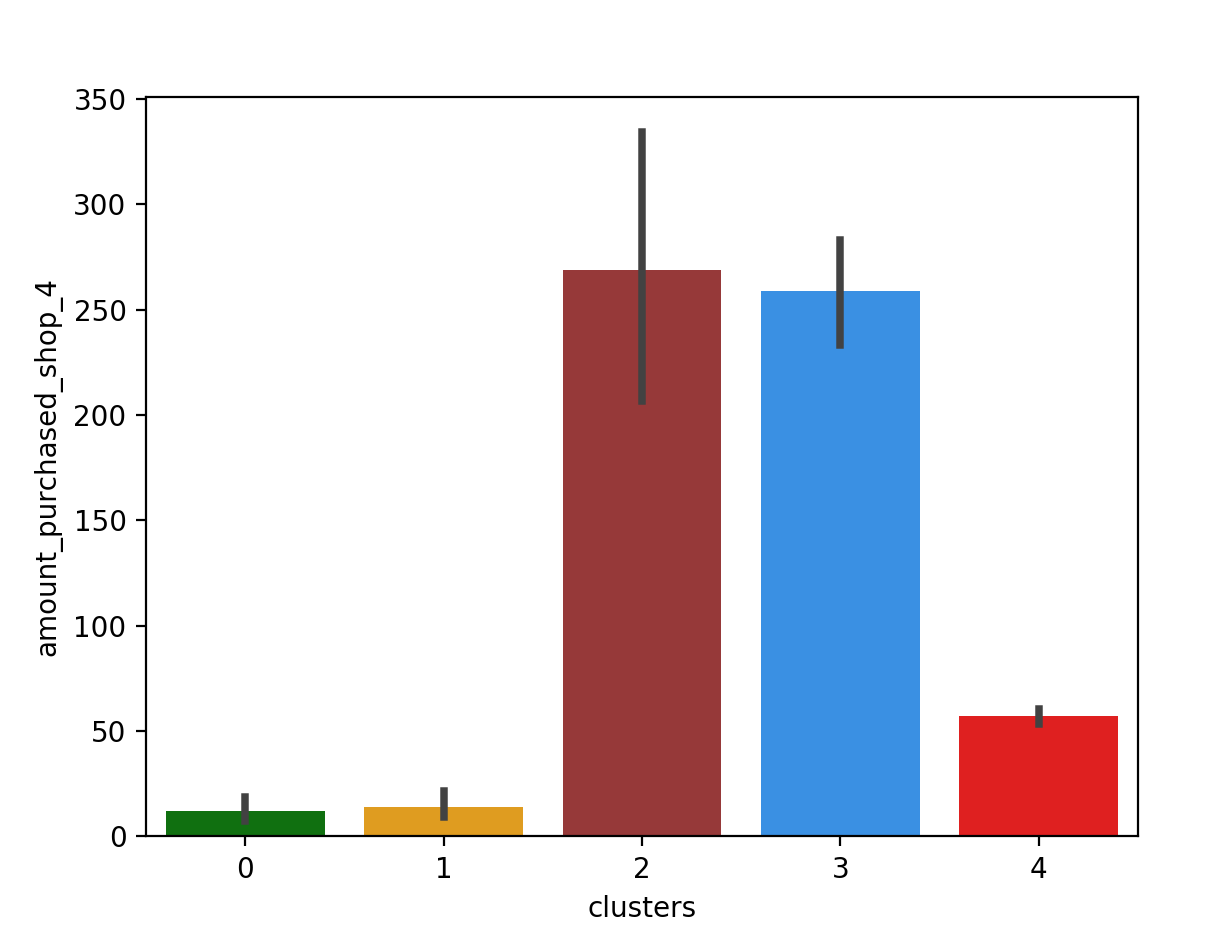
\includegraphics[scale=0.20] {cluster_shop4.png}
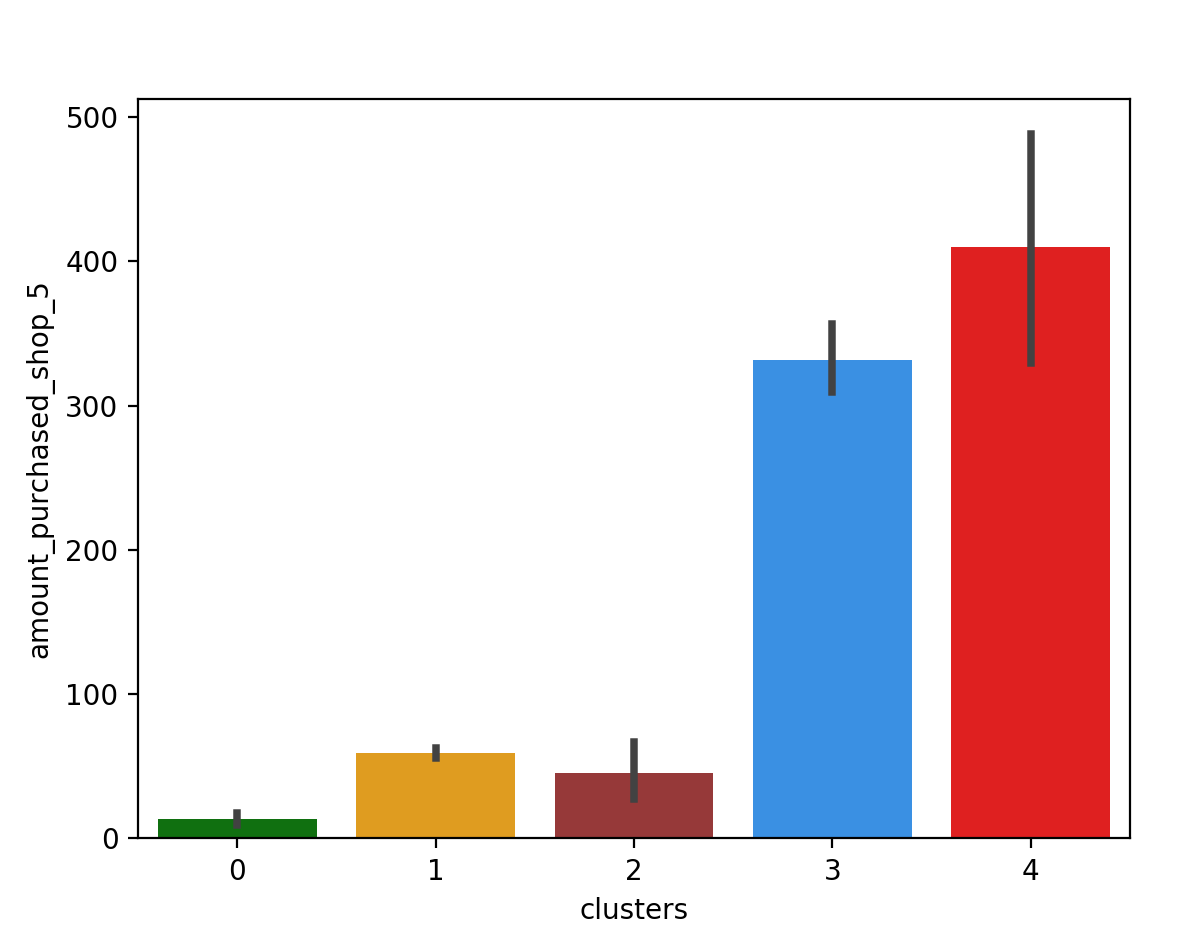
\includegraphics[scale=0.20] {cluster_shop5.png}
\end{center}

\noindent
Ainsi dans cette étude, la segmentation des clients peut être faite en se basant sur les magasins. Avec les données à notre disposition, nous ne pouvons pas pousser l'analyse plus loin. Dans un cas pratique en entreprise par exemple, une étude plus approfondie  peut être menée au sein de chaque magasin en ciblant les individus de clusters identifiés ci-dessus qui y viennent afin de cerner davantage leurs attentes.

\vspace{10 mm}

%###########################################################################################################################################
%###########################################################################################################################################
%###########################################################################################################################################
%###########################################################################################################################################



\nocite{XIN2011}
\nocite{OUM2016}
\nocite{FAB2018}

\renewcommand\bibname{Références}
\bibliographystyle{plain-fr}
\bibliography{biblio}
\addcontentsline{toc}{section}{Références}





\end{document}